% Turkish-CBE manuscript — entry point (see Appendix C.2, "Rebuilding the manuscript").
% Compile: latexmk -xelatex main.tex   (XeLaTeX + BibTeX; no model API,
% model weights, or experiment execution is required).
\documentclass[11pt]{article}

\usepackage[a4paper,margin=2.6cm,headheight=14pt]{geometry}
\usepackage{fontspec}
\usepackage{unicode-math}
\setmainfont{texgyretermes}[
  Extension=.otf,
  UprightFont=*-regular,
  BoldFont=*-bold,
  ItalicFont=*-italic,
  BoldItalicFont=*-bolditalic]
\setmathfont{texgyretermes-math.otf}
\setmonofont[Scale=0.88]{DejaVuSansMono}[
  Extension=.ttf,
  UprightFont=*,
  BoldFont=*-Bold]

\usepackage{amsmath}
\usepackage{amsthm}
\usepackage{booktabs}
\usepackage{graphicx}
\usepackage{microtype}
\usepackage{xcolor}
\usepackage{tikz}
\usetikzlibrary{positioning,arrows.meta,calc}
\usepackage{fancyhdr}
\usepackage[round]{natbib}
\usepackage{caption}
\usepackage{enumitem}
\usepackage[colorlinks=true,allcolors=linkblue,unicode]{hyperref}

\definecolor{linkblue}{HTML}{1F5C99}
\definecolor{headingblue}{HTML}{234E70}
\definecolor{stageblue}{HTML}{EAF1FB}
\definecolor{stageborder}{HTML}{2A78D6}
\definecolor{bandgreen}{HTML}{EAF6EF}
\definecolor{bandborder}{HTML}{1BAF7A}
\definecolor{exgray}{HTML}{F7F7F5}
\definecolor{mutedink}{HTML}{555555}

\usepackage{sectsty}
\allsectionsfont{\color{headingblue}}

\captionsetup{font=small,labelfont=bf}

\newtheorem{proposition}{Proposition}

\pagestyle{fancy}
\fancyhf{}
\fancyhead[L]{\small Turkish-CBE}
\fancyhead[R]{\small Reasoning accuracy and morphosyntactic robustness}
\fancyfoot[C]{\small\thepage}
\renewcommand{\headrulewidth}{0.4pt}

\newcommand{\inval}{\ensuremath{\bot}}

\title{\textbf{Turkish-CBE: Evaluating Logical Reasoning Accuracy\\
and Morphosyntactic Robustness in Large Language Models}\\[1.2ex]
\large A Controlled Turkish--English Benchmark with Correctness-Aware\\
\large Robustness Evaluation}

\author{Müge Oluçoğlu\\
\small İzmir Bakırçay University\\
\small ORCID: 0000-0002-0137-5854\\
\small \texttt{muge.olucoglu@bakircay.edu.tr}
\and
Okan Bursa\textsuperscript{*}\\
\small İzmir Bakırçay University\\
\small ORCID: 0000-0002-5958-0279\\
\small \texttt{okan.bursa@bakircay.edu.tr}\\
\small \textsuperscript{*}Corresponding author}

\date{\small 30 October 2026}

\begin{document}
\maketitle
\thispagestyle{empty}

\begin{abstract}
\noindent
Accuracy on a single language and a single formulation is an incomplete account of logical reasoning
reliability: a model may answer correctly only under one grammatical realization of a problem, or may
appear stable merely by repeating a biased answer. We present Turkish-CBE, a deterministic, reproducible
benchmark that renders the same latent ordering problem as matched Turkish and English prompts and as
answer-preserving Turkish presentation transformations (constituent order, converse constructions,
case/possessive alternatives), with exact symbolic answers, controlled entity counts and query distances,
and split-level separation of latent orders. A correctness-aware evaluation decomposes paired outcomes
into robust correctness, shared error, and presentation dependence on declared denominators,
distinguishing correct consistency from constant-response invariance. We report an exploratory evaluation
of GPT-4o and the Qwen2.5 instruct family (0.5B--14B; 16,618 matched prompts per model in a supplemental
quantized sweep). Sub-7B models are near-constant responders whose perfect invariance carries no
competence; discrimination emerges in English before Turkish; and a truth-preserving Turkish
constituent-order alternative (P3) reduces query-matched accuracy in the 14B model by 38.1 percentage
points (paired difference $-0.381$; 95\% cluster-bootstrap CI $[-0.418, -0.344]$), echoing GPT-4o's pilot
collapse to 36.9\%. A completed two-reviewer linguistic assessment of 360 sampled stimuli found unanimous
semantic-equivalence judgments within the reviewed sample, identified one construction excluded on
grammaticality grounds---after which the P3 reduction persists at 40.8 percentage points---and documented
disagreement regarding naturalness. Reasoning reliability should therefore be evaluated jointly over accuracy and
meaning-preserving presentation robustness; confirmatory frozen-test evaluation remains future work.
\end{abstract}

\vspace{0.6ex}
\noindent\textbf{Keywords:} large language models; logical reasoning evaluation; Turkish;
morphosyntax; cross-lingual evaluation; robustness; paired evaluation design; reproducibility;
benchmark construction; chance-corrected agreement

\section{Introduction}

A logical conclusion can remain unchanged when its premises are reordered, a relation is expressed through
its converse, or a language uses a different grammatical realization. A model that changes its answer under
such transformations presents a different evaluation problem from a model that consistently reaches the
wrong conclusion, and both differ from a model that appears stable only because it repeats a biased answer.
Aggregate accuracy on a single linguistic realization obscures all three distinctions: equal scores can
conceal failures on different instances, and high agreement can arise without any competence at all.
Behavioral tests and consistency evaluations therefore complement conventional task-level scores
\citep{ribeiro2020checklist, elazar2021pararel}.

Turkish offers an unusually well-controlled setting for making these distinctions measurable. It expresses
grammatical relations through productive suffixation and morphophonological alternations, and permits
constituent-order choices whose discourse effects a literal translation does not capture; computational
descriptions of Turkish morphology formalize the interaction between morphotactics and phonological
realization \citep{oflazer1994turkish}. These properties supply a family of \emph{answer-preserving}
transformations (premise reordering, converse constructions, constituent-order alternatives, and case or
possessive variants) that can be applied to the same underlying problem. We treat Turkish as a source
of controlled variation, not as a language presumed intrinsically harder for logical reasoning.

Existing resources do not answer how equivalent Turkish formulations affect transitive ordering inference.
General logical reasoning benchmarks \citep{yu2020reclor, liu2020logiqa, han2024folio} vary surface form
and content together; multilingual reasoning evaluations \citep{shi2023mgsm} compare independently sampled
items across languages; Turkish morphological-competence and minimal-pair benchmarks
\citep{ismayilzada2025morphology, basar2025turblimp, basar2026morphologyaware} intentionally manipulate
acceptability rather than holding the answer fixed; and paraphrase-consistency and metamorphic evaluations
\citep{elazar2021pararel, segura2016metamorphic} motivate, but do not provide, a matched bilingual ordering
design with exact answers. Competence-Based Evaluation (CBE) treats correctness across presentations of a
parameterized problem family as a behavioral requirement \citep{jiang2026cbe}; we adopt this framing and
extend it to Turkish--English matching, morphosyntactic interventions, lexical measurements, and
query-distance controls.

Turkish-CBE renders each latent strict total order as matched Turkish and English prompts and as controlled
Turkish presentation transformations, with exact symbolic answers, explicit entity-count and query-distance
factors, and split-level separation of latent orders. On top of this design, a correctness-aware analysis
decomposes paired outcomes on jointly valid support into robust correctness ($R$), shared-wrong agreement
($D$), and presentation dependence ($U$), reported together with raw invariance, a chance-corrected
agreement coefficient, valid-pair coverage, and strict all-planned robustness
(Section~\ref{sec:statistics}). These quantities are complementary: invariance alone cannot separate
correct consistency from stable error, and accuracy alone cannot reveal presentation dependence.

The framework is exercised by completed exploratory experiments. A registered pilot evaluates
Qwen2.5-0.5B-Instruct and \texttt{gpt-4o-2024-08-06} on matched prompts (Section~\ref{sec:pilot}); a
supplemental quantized local sweep evaluates four Qwen2.5 scales (0.5B--14B) on 16,618 matched prompts each
across all nine relation families (Section~\ref{sec:p1-local}); and a two-reviewer Turkish linguistic
assessment of 360 sampled stimuli was completed after these runs (Section~\ref{sec:review}); it found
unanimous semantic-equivalence judgments within the reviewed sample, identified one construction requiring
grammaticality-based exclusion, and documented contested naturalness.

This article makes three principal contributions:
\begin{enumerate}[leftmargin=1.6em]
  \item \textbf{A controlled bilingual reasoning benchmark.} A deterministic, reproducible framework that
  holds the latent problem, gold answer, names, and query geometry fixed while varying language and Turkish
  presentation, supporting more controlled comparisons than independently sampled multilingual test sets.
  The design does not claim to eliminate every linguistic or tokenization confounder; it makes the remaining
  ones explicit and measurable.
  \item \textbf{Correctness-aware presentation robustness.} A denominator-aware paired decomposition that
  separates correctness from response stability. Its components are related to existing agreement and
  paired-outcome methods rather than constituting a new statistical theory; their joint presentation is what
  carries the evaluation content. The constant-response behavior of the smaller evaluated models provides a
  concrete empirical demonstration that high response invariance does not indicate reasoning competence.
  \item \textbf{An empirical characterization of linguistic presentation sensitivity.} Within the evaluated
  models, datasets, and settings: model-scale differences in discriminative accuracy, English--Turkish
  performance differences, strong sensitivity to the P3 constituent-order presentation, complexity-dependent
  degradation, naming-condition effects, and the distinction between correct consistency and
  constant-response invariance. These are findings about the evaluated systems, not generalizations to all
  large language models.
\end{enumerate}

Turkish-CBE addresses five research questions. RQ1 concerns the paired Turkish--English accuracy
difference; RQ2 sensitivity to answer-preserving Turkish presentations; RQ3 the separation of entity count
from query distance and query type; RQ4 associations among relation vocabulary, corpus frequency,
tokenization, and predicted-answer bias; RQ5 whether reasoning prompting or optional adaptation improves
correct consistency as well as accuracy. The completed exploratory evidence bears on RQ1--RQ3 (and supplies
RQ4 diagnostics), while confirmatory answers to all five---and any RQ5 adaptation effect---are reserved for
the preregistered frozen-test design (Section~\ref{sec:future}).

\section{Related Work}

\subsection{Logical reasoning benchmarks and controlled generation}

Natural-language reasoning benchmarks differ in their source material and the inferential structures they
expose. ReClor and LogiQA evaluate reasoning-oriented reading comprehension \citep{yu2020reclor,
liu2020logiqa}. FOLIO connects natural-language arguments to first-order logical representations
\citep{han2024folio}. Their task diversity is valuable, but a change in the language or surface form of an
item need not preserve all other evaluation conditions. Turkish-CBE instead fixes a narrow ordering family
so that the latent question and its answer can be held constant across presentations.

Generated benchmarks provide complementary structural control. CLUTRR tests relational reasoning from text
\citep{sinha2019clutrr}; RuleTaker studies reasoning over natural-language rule bases
\citep{clark2020ruletaker}; and ProofWriter adds generated implications, proofs, and abductive statements
\citep{tafjord2021proofwriter}. PrOntoQA supports formal analysis of reasoning chains
\citep{saparov2023prontoqa}. These precedents show why explicit structure and an oracle are useful. Our
contribution is not the invention of generated reasoning data; it is their use within a matched Turkish
presentation design, with input size and latent proof distance separately recorded.

\subsection{Robustness, metamorphic relations, and consistency}

Metamorphic testing specifies relations between outputs under controlled input transformations
\citep{segura2016metamorphic}. CheckList applies behavioral test design to language technologies
\citep{ribeiro2020checklist}. ParaRel studies consistency across paraphrased factual queries
\citep{elazar2021pararel}; factual cloze consistency is distinct from deductive ordering, but it motivates
separating correctness from stability. CBE combines a scalable latent family with an explicit
answer-preservation requirement \citep{jiang2026cbe}. We retain that requirement and add Turkish-specific
interventions and missing-response accounting.

Controlled perturbations in arithmetic also motivate careful interpretation. GSM-Symbolic evaluates
variation in mathematically structured problems \citep{mirzadeh2025gsm}. Its task differs from ordering, so
neither its numerical findings nor a particular mechanistic explanation is imported here. A presentation
effect can reflect parsing, retrieval, lexical priors, or inference; behavioral inconsistency alone does not
distinguish those causes.

\subsection{Multilingual reasoning and Turkish linguistic evaluation}

MGSM investigates multilingual chain-of-thought arithmetic reasoning \citep{shi2023mgsm}. Turkish is not
one of its evaluated languages, and arithmetic success cannot validate Turkish ordering templates. A
multilingual ordering benchmark must therefore establish its own linguistic equivalence and matched
sampling.

Turkish morphology has long motivated explicit computational modeling \citep{oflazer1994turkish}.
Morphological compositionality experiments expose limitations in combining morphemes productively
\citep{ismayilzada2025morphology}. TurBLiMP evaluates Turkish minimal-pair acceptability
\citep{basar2025turblimp}, whereas morphology-aware syntax evaluation examines how surface factors can bias
judgments \citep{basar2026morphologyaware}. Those tasks are complementary to ours: minimal-pair
grammaticality contrasts often intentionally change acceptability, while Turkish-CBE requires grammatical
alternatives that preserve truth and the gold answer. Native-speaker adjudication remains necessary despite
deterministic rendering.

\subsection{Tokenization, frequency proxies, and reasoning interventions}

Tokenizer quality and language coverage can affect multilingual model behavior \citep{rust2021tokenizer}.
Token-length inequalities also matter for access costs and processing budgets \citep{ahia2023languages,
petrov2023tokenizers}. These observations justify measuring tokenization rather than assuming equal cost
for matched text. They do not establish a causal tokenization explanation for a logical error. Corpus
frequency is likewise a proxy with explicit genre, annotation, and segmentation limits; our independent
resource is the locked BOUN treebank release \citep{turk2022boun}.

Chain-of-thought prompting and self-consistency are distinct interventions \citep{wei2022cot,
wang2023selfconsistency}. Self-consistency aggregates sampled responses to one input; presentation
invariance compares different inputs that preserve the same answer. Moreover, generated explanations need
not faithfully report the causes of an answer \citep{turpin2023unfaithful}. Parameter-efficient adaptation
with LoRA \citep{hu2021lora} and group-relative policy optimization \citep{shao2024deepseekmath} motivate
optional training arms, but their success elsewhere provides no evidence that our unrun adapters improve
Turkish reasoning.

\section{Methodology}

\subsection{Latent structure, oracle, and query geometry}

Let a latent instance be a strict total order
\begin{equation}
  z = \bigl(e_{\sigma(1)} \prec e_{\sigma(2)} \prec \cdots \prec e_{\sigma(n)}\bigr),
  \qquad |E| = n.
  \label{eq:latent}
\end{equation}
The frozen size grid is $n \in \{4, 8, 16, 32, 64, 128, 256, 512, 1024\}$. The generator draws a
permutation of unique entities and emits the $n-1$ adjacent comparisons. A language-independent rank map
$r_z : E \to \{1, \ldots, n\}$ defines the exact answer to a forward query:
\begin{equation}
  y^{*}(z, a, b, \prec) = \mathbf{1}\{r_z(a) < r_z(b)\}.
  \label{eq:oracle}
\end{equation}
The inverse relation reverses the inequality. A separate graph check validates the chain and its entailed
comparisons. Stable, versioned seed derivation separates naming, permutation, premise order, and query
selection, so introducing a new presentation condition does not alter previously defined latent instances.

Endpoint queries compare the first and last positions. Internal queries sample two positions strictly
inside the chain. Distance-controlled queries fix
\begin{equation}
  d = |r_z(a) - r_z(b)|,
  \label{eq:distance}
\end{equation}
with both positions internal. Thus their feasible distances satisfy $1 \le d \le n-3$; the retained
power-of-two grid is intersected with that range. This is narrower than merely requiring $d < n$. At
$n = 4$, an internal pair necessarily has $d = 1$, so internal and distance-controlled conditions can share
geometry. Such repetitions are not independent evidence.

A longer endpoint chain does not prove deeper inference. The source and sink can be identified by their
incident-edge signatures under the chain assumptions, avoiding a full transitive derivation. Entity count
measures input and presentation load; $d$ measures latent graph distance, not observed model computation.
We therefore retain endpoint and internal/distance strata and do not treat their pooled score as an
inference-depth curve.

\begin{table}[t]
  \centering
  \caption{Turkish presentation factors. P0 denotes the canonical form. The general matched equivalent
  condition is retained separately from isolated ablations.}
  \label{tab:presentations}
  \small
  \begin{tabular}{@{}llp{0.42\linewidth}@{}}
    \toprule
    Factor & Operation & Interpretation control \\
    \midrule
    P0 & Canonical grammatical realization & Baseline; identical latent query. \\
    P1 & Reorder premises and names list & Preserve words and predicates. \\
    P2 & Swap arguments and use inverse relation & Preserve the asserted comparison. \\
    P3 & Alternative constituent construction & Truth preservation does not imply identical discourse
         preference. \\
    P4 & Valid case/possessive morphology alternatives & Label additional syntax/lexical changes
         explicitly. \\
    P5 & Combine several operations & Compound perturbation; no pure morphology attribution. \\
    P6 & Optional controlled negation & Excluded from the frozen core; requires strict-order proof. \\
    \bottomrule
  \end{tabular}
\end{table}

\subsection{Language realization and equivalent presentations}

A renderer $\pi_{\ell,p,v,c}$ maps a latent query to language $\ell$, presentation $p$, relation vocabulary
$v$, and name control $c$. Its formal contract is
\begin{equation}
  \mathcal{N}\bigl(\pi_{\ell,p,v,c}(z)\bigr) = \mathcal{N}(z),
  \qquad
  y^{*}\bigl(\pi_{\ell,p,v,c}(z)\bigr) = y^{*}(z),
  \label{eq:contract}
\end{equation}
where $\mathcal{N}$ is the closed-grammar logical normal form. Converse realization swaps arguments and
uses the inverse predicate; for example, $a \prec b$ is realized as either a forward statement about $a$ or
an inverse statement about $b$. Premise order and names-list order are independent surface factors.

The inventory contains nine relations from spatial, temporal, comparative, and ranking families. Spatial
relations have explicitly linear positional interpretations. Turkish realization selects
genitive/possessive or ablative constructions as appropriate, handles proper-name apostrophes, and applies
vowel and consonant harmony. The reference to Turkish morphological theory \citep{oflazer1994turkish}
motivates these constraints; it does not certify our implementation. Table~\ref{tab:presentations}
separates operational transformations from linguistic claims.

\subsection{Semantic validation and human adjudication}

Automatic validation checks distinct entities, chain consistency, premise truth, query distance,
normal-form equivalence, and oracle agreement. Rendering and parsing are partly based on shared linguistic
code, creating a common-mode failure risk. Passing a round trip establishes a contract within the
implemented grammar; it is not an independent proof of naturalness or unrestricted Turkish equivalence.

Two independent Turkish-proficient reviewers must judge grammaticality, naturalness, semantic equivalence,
and morphology, with disagreements resolved before an approved review record is issued. The operational
large-run gate requires at least 100 distinct reviewed Turkish prompts, at least 20 in each selected
relation--presentation--name template cell, and coverage of every requested size and query type. This is
sampled review, not exhaustive review of every cross-cell. Existing automatic checks and an unfilled review
sheet do not constitute human approval. A review of this form was executed on a stratified sample of the
evaluated prompt population; its instrument, predeclared inclusion policy, and outcomes are reported in
Section~\ref{sec:review}. Work on Turkish minimal pairs reinforces the need to separate
grammatical evaluation from logical labels \citep{basar2025turblimp, basar2026morphologyaware}.

\begin{figure}[t]
  \centering
  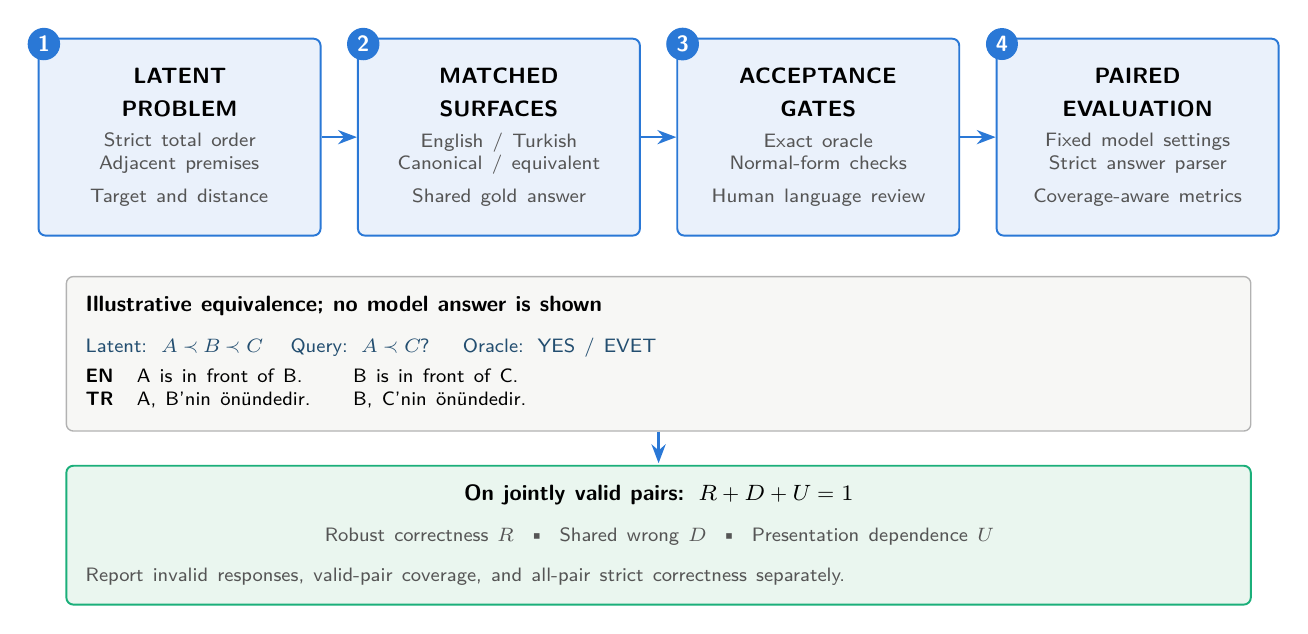
\begin{tikzpicture}[
      font=\sffamily,
      stage/.style={
        draw=stageborder, fill=stageblue, rounded corners=2.5pt, line width=0.7pt,
        minimum height=2.5cm, text width=3.3cm, align=center, inner sep=4pt},
      stagenum/.style={
        fill=stageborder, text=white, font=\sffamily\bfseries\footnotesize,
        circle, inner sep=1.6pt, minimum size=11pt},
      flow/.style={-{Stealth[length=2.4mm]}, line width=0.9pt, draw=stageborder},
      lbl/.style={font=\sffamily\bfseries\footnotesize, align=center},
      body/.style={font=\sffamily\scriptsize, align=center, text=mutedink},
    ]
    % Stage cards
    \node[stage] (s1) at (0,0)
      {\textbf{\footnotesize LATENT}\\ \textbf{\footnotesize PROBLEM}\\[3pt]
       {\scriptsize\color{mutedink} Strict total order\\ Adjacent premises\\ Target and distance}};
    \node[stage, right=0.45cm of s1] (s2)
      {\textbf{\footnotesize MATCHED}\\ \textbf{\footnotesize SURFACES}\\[3pt]
       {\scriptsize\color{mutedink} English / Turkish\\ Canonical / equivalent\\ Shared gold answer}};
    \node[stage, right=0.45cm of s2] (s3)
      {\textbf{\footnotesize ACCEPTANCE}\\ \textbf{\footnotesize GATES}\\[3pt]
       {\scriptsize\color{mutedink} Exact oracle\\ Normal-form checks\\ Human language review}};
    \node[stage, right=0.45cm of s3] (s4)
      {\textbf{\footnotesize PAIRED}\\ \textbf{\footnotesize EVALUATION}\\[3pt]
       {\scriptsize\color{mutedink} Fixed model settings\\ Strict answer parser\\ Coverage-aware metrics}};
    \node[stagenum] at ($(s1.north west)+(0.08,-0.08)$) {1};
    \node[stagenum] at ($(s2.north west)+(0.08,-0.08)$) {2};
    \node[stagenum] at ($(s3.north west)+(0.08,-0.08)$) {3};
    \node[stagenum] at ($(s4.north west)+(0.08,-0.08)$) {4};
    \draw[flow] (s1) -- (s2);
    \draw[flow] (s2) -- (s3);
    \draw[flow] (s3) -- (s4);

    % Example panel
    \node[draw=mutedink!45, fill=exgray, rounded corners=2.5pt, line width=0.5pt,
          text width=14.55cm, inner sep=7pt, below=0.5cm of $(s2.south)!0.5!(s3.south)$, anchor=north]
      (ex) {
        {\footnotesize\bfseries Illustrative equivalence; no model answer is shown}\\[3pt]
        {\scriptsize\color{headingblue}
          Latent: $A \prec B \prec C$ \quad Query: $A \prec C$? \quad Oracle: YES / EVET}\\[3pt]
        {\scriptsize
          \begin{tabular}{@{}l@{\hspace{1.2em}}l@{\hspace{2.2em}}l@{}}
            \textbf{EN} & A is in front of B. & B is in front of C. \\
            \textbf{TR} & A, B'nin önündedir. & B, C'nin önündedir. \\
          \end{tabular}}
      };
    \draw[flow] (ex.south) -- ++(0,-0.4);

    % Metrics band
    \node[draw=bandborder, fill=bandgreen, rounded corners=2.5pt, line width=0.7pt,
          text width=14.55cm, inner sep=7pt, below=0.42cm of ex, anchor=north] (band) {
        \centering
        {\footnotesize\bfseries On jointly valid pairs: $R + D + U = 1$}\\[2.5pt]
        {\scriptsize\color{mutedink}
          Robust correctness $R$ \;\textbullet\; Shared wrong $D$ \;\textbullet\;
          Presentation dependence $U$}\\[2.5pt]
        {\scriptsize\color{mutedink}
          Report invalid responses, valid-pair coverage, and all-pair strict correctness separately.}
      };
  \end{tikzpicture}
  \caption{Turkish-CBE architecture and an illustrative bilingual realization. The diagram describes the
  evaluation design, not observed model accuracy.}
  \label{fig:architecture}
\end{figure}

\subsection{Bilingual matching, names, and split integrity}

Turkish and English records share the latent-order identifier, query target, query direction, gold label,
and presentation plan. The \texttt{native\_shared} control uses the same native Unicode spelling in both
languages. \texttt{en\_transliterated} changes only the English labels, retaining native Turkish spelling
and morphology. \texttt{symbolic\_shared} assigns identical symbolic labels in both languages.
Consequently, the transliterated arm intentionally changes naming together with language; it is a
naming-sensitivity control, not a pure language contrast. The shared-name arms support the cleaner matched
comparison. They do not remove all differences in tokenizer vocabulary, instructions, or response labels.
All derivatives of a latent order are assigned to one split before rendering; changing the vocabulary cannot
move the same instance from training into test.

The upstream generator supports several entity inventories, but the frozen paired bank analyzed here uses
the Turkish-name source inventory before alias expansion; a fully crossed synthetic-name experiment is not
established by these counts. The unit of independence is the source order, not a prompt record or
comparison cell. The total-order family is structurally isomorphic under renaming: exact train/test
instance separation is not separation of abstract reasoning algorithms or a guarantee against external
pre-training contamination. The current frozen grid crosses three name controls, nine relations, and nine
language/presentation conditions: two English conditions and seven Turkish conditions (canonical, general
equivalent, and P1--P5). This produces $3 \times 9 \times 9 = 243$ prompt identities for each source query.
Optional negation is not silently included in that expansion.

\section{Correctness, Invariance, and Statistical Inference}
\label{sec:statistics}

\subsection{Denominators and the paired outcome decomposition}

For $N$ planned matched presentation pairs, let $a_{ik} \in \{0, 1, \inval\}$ be the strictly parsed answer
to presentation $k \in \{0, 1\}$, where $\inval$ denotes invalid or missing output. Marginal correctness is
$C_{ik} = \mathbf{1}\{a_{ik} = y_i^{*}\}$, with invalid answers wrong. Define
$V_i = \mathbf{1}\{a_{i0} \ne \inval,\, a_{i1} \ne \inval\}$ and $M = \sum_i V_i$. The marginal accuracies
and valid-pair coverage are
\begin{equation}
  \widehat{A}_k = \frac{1}{N} \sum_{i=1}^{N} C_{ik},
  \qquad
  \widehat{v} = \frac{M}{N}.
  \label{eq:marginals}
\end{equation}
For $M > 0$, the paired CBE quantities use exactly the same jointly valid support:
\begin{align}
  \widehat{R} &= \frac{1}{M} \sum_i V_i\, C_{i0} C_{i1}, \label{eq:R}\\
  \widehat{D} &= \frac{1}{M} \sum_i V_i\, (1 - C_{i0})(1 - C_{i1}), \label{eq:D}\\
  \widehat{U} &= \frac{1}{M} \sum_i V_i\, \mathbf{1}\{C_{i0} \ne C_{i1}\}. \label{eq:U}
\end{align}
Consequently,
\begin{equation}
  \widehat{R} + \widehat{D} + \widehat{U} = 1,
  \qquad
  \widehat{A}_{\mathrm{valid}} = \widehat{R} + \widehat{U}/2,
  \qquad
  \widehat{I} = \widehat{R} + \widehat{D}.
  \label{eq:identities}
\end{equation}
Here $\widehat{A}_{\mathrm{valid}}$ is the mean of the two accuracies \emph{on jointly valid pairs}. It is
not automatically $(\widehat{A}_0 + \widehat{A}_1)/2$ on the full planned sample. Binary gold labels shared
within each pair imply that $D$ is shared-wrong agreement, whereas $U$ is presentation dependence.

For $N > 0$ and $M > 0$, strict robust correctness retains all planned pairs:
\begin{equation}
  \widehat{R}_{\mathrm{strict}} = \frac{\sum_i V_i\, C_{i0} C_{i1}}{N} = \widehat{v}\, \widehat{R}.
  \label{eq:strict}
\end{equation}
The equality exposes selective coverage directly. It does not assert that marginal accuracy equals coverage
times valid-pair accuracy: pairs with one valid, correct answer can still contribute to a marginal. Both
response-level invalid rates and pair coverage must accompany every conditional profile. If $M = 0$ and
$N > 0$, strict robustness is zero while conditional $R$ is undefined; the product identity is used only
when $R$ is defined. Empty conditional denominators are undefined, not zero.

\subsection{Chance correction and its interpretation}

At a fixed complexity and declared model/condition stratum, define $q$ as the pooled YES/EVET rate over the
$2M$ jointly valid answers. The retained CBE reference is
\begin{equation}
  I_e = q^2 + (1 - q)^2,
  \qquad
  \kappa_{\mathrm{CBE}} = \frac{\widehat{I} - I_e}{1 - I_e}.
  \label{eq:kappa}
\end{equation}
Constant outputs make $I_e = 1$, so the coefficient is undefined. High raw agreement from a constant answer
is therefore not evidence of competence. The chance correction is related to the general idea of agreement
beyond chance \citep{cohen1960kappa}, but its pooled reference is not identical to the separate-marginal
reference in conventional Cohen kappa. Appendix~\ref{app:identities} derives the difference. Neither
reference identifies an internal reasoning mechanism or proves stochastic independence.

A valid-pair mean accuracy alone bounds but does not determine robustness. From the nonnegative outcome
masses,
\begin{equation}
  \max(0,\, 2A_{\mathrm{valid}} - 1) \le R \le A_{\mathrm{valid}}.
  \label{eq:bounds}
\end{equation}
Likewise, invariance cannot identify the division between correct and shared-wrong agreement. These
algebraic observations explain why accuracy, $R$, $D$, $U$, coverage, and chance correction should be
presented jointly rather than ranked as interchangeable notions of reliability.

\subsection{Paired inference, dependence, and multiplicity}

The primary cross-language accuracy effect is
\begin{equation}
  \widehat{\Delta}_{\mathrm{TR-EN}} = N^{-1} \sum_i \bigl(C_{i,\mathrm{TR}} - C_{i,\mathrm{EN}}\bigr),
  \label{eq:delta}
\end{equation}
using identical planned coordinates and counting invalid answers wrong. Effects are evaluated within
declared model, size, query-type/distance, relation, presentation, and name-control strata. Any pooled
summary must specify whether it weights derived queries, latent orders, or size levels; those are different
estimands. Paired McNemar inference \citep{mcnemar1947} compares discordant correctness outcomes when
matched units are independent. The exact conditional version uses a binomial reference on discordant pairs.
Repeated queries or presentations from one latent order violate ordinary row-level independence; such rows
require cluster-aware uncertainty rather than an unqualified McNemar $p$-value.

Confidence intervals use 2,000 matched latent-order bootstrap replicates, preserving every dependent
query/presentation record and resampling within declared size strata. This extends the resampling principle
\citep{efron1979bootstrap} to the clustered design \citep{field2007clustered}. Wilson intervals
\citep{wilson1927} are useful binomial summaries for $R$ only under an appropriate independent-Bernoulli
interpretation; when rows share latent orders, dependence-aware bootstrap intervals carry the inferential
interpretation. Intervals are pointwise, not simultaneous bands.

Holm correction \citep{holm1979} applies within predeclared model/design/metric families, with missing
planned hypotheses retaining their correction slots. The implementation is not study-wide familywise
control across every size, relation, distance, and intervention. Confirmatory families must be specified
before outcomes are observed. For base--adapter comparisons, all-planned accuracy, strict $R$, and coverage
are primary; common-four-valid differences in conditional $R$, invariance, and kappa are explicitly labeled
sensitivity analyses and report both arms' valid support.

\subsection{Lexical associations and identifiable effects}

For each relation direction, the predicted YES/EVET rate is the number of parsed affirmative answers divided
by the number of parsed responses in that direction. Its denominator, planned gold-label balance, and
invalid rate must be shown together. This descriptive rate may use lone valid responses; it is distinct from
the pooled $q$ in Equation~\eqref{eq:kappa}, which uses jointly valid pairs only. A direction-specific
accuracy change and invariance change need not agree.

Frequency--accuracy and tokenization--invariance analyses were executed on the pilot outcomes
(Section~\ref{sec:pilot}) but remain unidentified there, because a single relation family supplies at most
two lexical units per cell. Spearman association \citep{spearman1904} can summarize monotone relations, but
a handful of repeated lexical units does not create independent observations through prompt replication. A
multivariable specification may include model, relation family, $\log_2 n$, query distance, and prompt
length, with uncertainty clustered by latent order and appropriate attention to lexical reuse. Saturated
model-by-vocabulary effects may absorb all between-term frequency variation; unsupported or collinear fits
must remain unavailable, and the retained pilot outputs record them as such rather than as coefficients.

We distinguish a total paired language contrast from an estimate adjusted for token length. Length may lie
on a pathway by which language changes the presented input, so adjustment changes the question rather than
automatically correcting a nuisance. These are descriptive associational analyses, not identification of a
causal frequency or morphology effect. No lexical-association coefficient is promoted to a finding in the
current article; the executed pilot specifications are retained with their explicit unidentifiability
statuses.

\section{Experimental Design and Reproducibility}

\subsection{Research questions and registered contrasts}

\begin{table}[t]
  \centering
  \caption{Research questions and the measurements needed to answer them. Exploratory estimates of the
  RQ1--RQ3 readouts (and RQ4 diagnostics) exist from the completed pilot and supplemental evaluations
  (Sections~\ref{sec:pilot}--\ref{sec:review}); confirmatory frozen-test estimates and the RQ5 adapter
  contrast remain pending.}
  \label{tab:rqs}
  \small
  \begin{tabular}{@{}lp{0.42\linewidth}p{0.40\linewidth}@{}}
    \toprule
    RQ & Matched contrast & Required readout \\
    \midrule
    RQ1 & English vs.\ Turkish at fixed latent query, names, and presentation &
      Paired accuracy difference, invalid rates, coverage. \\
    RQ2 & Turkish canonical vs.\ equivalent/P1--P5 &
      $R$, $D$, $U$, $I$, $\kappa$, strict $R$, support. \\
    RQ3 & Size and distance within each query type &
      Separate $n$ and $d$ profiles; endpoint/internal contrast. \\
    RQ4 & Relation terms and directions on identical instances &
      Frequency/token features, predicted YES rate, accuracy and invariance jointly. \\
    RQ5 & Direct vs.\ reasoning; base vs.\ trained adapter &
      Matched effects, common support, usage and compute budgets. \\
    \bottomrule
  \end{tabular}
\end{table}

Table~\ref{tab:rqs} connects each research question to a planned estimand. Four-cell balancing crosses
query direction and gold answer. Frozen test strata contain 200 source orders per size and 50 examples per
direction--gold cell; smaller pilot/development/training strata use approximately balanced 12/13 cells where
50 cannot be split equally. Derived presentations retain those source labels rather than creating additional
independent cases.

The recorded split generation seeds are 401 (training), 402 (development), 403 (pilot), and 404 (test),
with presentation seed 431. Seed derivation remains versioned and namespaced. The experiment matrix
separates English canonical/equivalent, Turkish canonical/equivalent, cross-language canonical,
cross-language equivalent, Turkish ablations, and endpoint-to-interior contrasts. The last changes the
queried proposition and may change the gold answer; it is a query-complexity comparison, not an
answer-preserving presentation pair. We therefore do not compute presentation invariance by blindly pairing
endpoint and internal answers as if they answered the same question.

\subsection{Prompts, parsers, and generation budgets}

The direct Turkish instruction asks the model to use the supplied premises and return only \texttt{EVET} or
\texttt{HAYIR}; the English control requests \texttt{YES} or \texttt{NO}. A strict language-specific parser
accepts only the specified form, records wrong-language outputs separately, and rejects contradictory or
extra answers. It does not search arbitrary response text for a convenient label. Reasoning conditions
instead require an unambiguous final-answer marker, with correctness determined by that answer rather than
by the explanation.

A run must record immutable model and tokenizer identities, provider/serving revision, sampling parameters,
seed where supported, system/user prompts, context and output budgets, reasoning setting, token usage,
truncation, and cost status. Model unavailability cannot silently select a replacement. Planned tokens are
not billed usage, and isolated-string token counts are not chat-template counts. Context failures, missing
completions, and invalid responses stay in planned-sample denominators.

Dry-runs estimate call counts before a small real pilot. Full evaluation requires an approved pilot; large
evaluations, including pilots or training evaluation exceeding 2,000 planned generation calls, also require
dataset- and scope-bound human linguistic review. Checkpointing and append-only raw records support
resumption without overwriting model evidence. An identical-prompt repeat control should accompany
stochastic or provider-nondeterministic settings, so cross-presentation disagreement is not automatically
attributed to linguistic variation. This is a prospective control, not a reported experiment. A local
journal establishes recorded lineage, not independent provider attestation. Two registered configurations
(Qwen2.5-0.5B-Instruct and \texttt{gpt-4o-2024-08-06}) were enabled by explicit user selection and executed
under this protocol (Section~\ref{sec:pilot}); the supplemental quantized sweep reuses the frozen prompts,
message construction, and strict parser outside the registered provider set and is labeled accordingly
(Section~\ref{sec:p1-local}). The execution-gate receipts for runs above the declared call threshold have
not been issued, so no run in this article carries confirmatory authorization.

\subsection{Reasoning and optional training interventions}

Direct answering, open stepwise prompting, structured normalization/direction/transitivity prompting, and
provider reasoning-effort controls are distinct arms. Their latent queries, gold labels, and sampling
conditions should be held constant where possible. Output budgets must be sufficient and recorded; changes
in budget can otherwise confound interpretation. CoT and sampled self-consistency \citep{wei2022cot,
wang2023selfconsistency} motivate interventions but are not the same as invariance across equivalent
presentations. Final-answer improvements do not establish explanation faithfulness
\citep{turpin2023unfaithful}.

Optional training compares a base model, SFT-LoRA, paired-presentation SFT, SFT with a consistency term,
correctness-only GRPO, and correctness-plus-consistency GRPO. LoRA supplies a parameter-efficient adaptation
mechanism \citep{hu2021lora}; GRPO is a group-relative policy optimization method introduced in mathematical
reasoning \citep{shao2024deepseekmath}. We do not claim to reproduce their original numerical results. The
proposed reward form is $r = \text{correctness} + 0.5\,\text{agreement bonus}$, with correctness monitored
independently. Under binary rewards, within-group advantage normalization can make an additive agreement
component ineffective; diagnostics of reward and normalized advantage are therefore necessary.

Training uses $n \le 128$, with larger-size and held-out-vocabulary evaluation kept separate. Latent
instances must be disjoint across training and test. English context words such as \emph{higher/lower} can
overlap even when relation terms are held out, so predicate novelty is not full-context novelty. Fair
comparison records example counts, actual training tokens, GPU time, steps, and trainable/update budgets;
equal steps do not equalize compute. The local Apple M1/16-GiB preparation machine has no CUDA device; the
training backend was validated on rented CUDA hardware by executed smoke-scale runs of all five arms under
the declared dependency pins (Section~\ref{sec:pilot}). These runs establish pipeline feasibility and
accounting only: no adapter has been performance-evaluated, and no adaptation improvement of any direction
is claimed in this article.

\section{Construction and Preprocessing Results}

The following results concern actual dataset inventories and retained corpus/tokenizer measurements. They
are not simulated model responses. Counts summarize the constructed collection; they are not random-sample
estimates of a population accuracy, so model-performance confidence intervals and significance tests are
inapplicable. The 33 split-by-size dataset records and the 236 native lexical publication records supply
every numerical display in this section.

\subsection{Dataset scale and the distinction between units}

The collection contains 3,000 latent orders, 23,200 source queries, 5,637,600 prompt identities, and
7,819,200 comparison cells (Table~\ref{tab:inventory}). Source-order allocation is 450 training, 450
development, 300 pilot, and 1,800 test orders. The training allocation spans the frozen size grid, while optional training selects only
$n \le 128$; split membership does not imply selection for optimization. These counts describe different
units: each source order supports multiple queries, and each query expands into 243
language/name/relation/presentation identities. Comparison cells additionally include matched contrasts and
endpoint-to-interior comparisons. They are not 7.8 million independent reasoning trials.

\begin{table}[t]
  \centering
  \caption{Verified dataset inventory. Orders are source chains; queries and presentations are dependent
  derivatives. Presentation counts describe the frozen design, not completed model calls.}
  \label{tab:inventory}
  \small
  \begin{tabular}{@{}lrrrr@{}}
    \toprule
    Split & Orders & Queries & Presentations & Pairing cells \\
    \midrule
    Training    &   450 &  3\,550 &   862\,650 & 1\,197\,450 \\
    Development &   450 &  3\,550 &   862\,650 & 1\,197\,450 \\
    Pilot       &   300 &  1\,900 &   461\,700 &   634\,500 \\
    Frozen test & 1\,800 & 14\,200 & 3\,450\,600 & 4\,789\,800 \\
    \midrule
    Total       & 3\,000 & 23\,200 & 5\,637\,600 & 7\,819\,200 \\
    \bottomrule
  \end{tabular}
\end{table}

\begin{figure}[t]
  \centering
  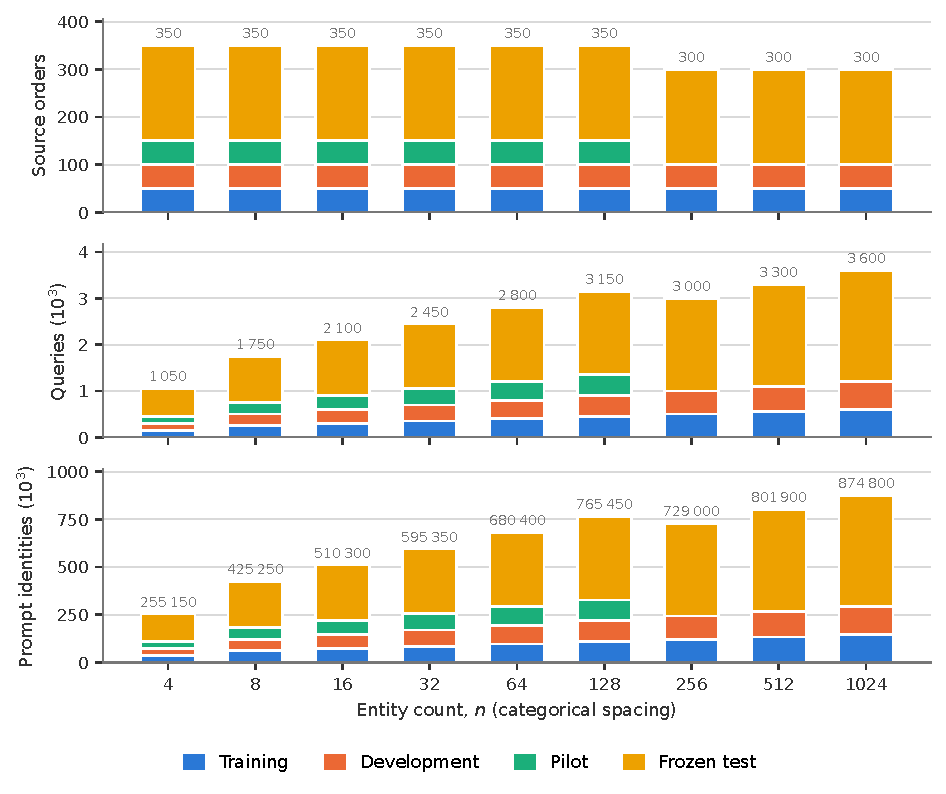
\includegraphics[width=\linewidth]{figures/manuscript/fig2_construction_counts.pdf}
  \caption{Verified construction counts by size and split. Source orders and derived queries/prompts are
  different units. This figure contains no model predictions.}
  \label{fig:construction}
\end{figure}

Figure~\ref{fig:construction} shows why entity count, independent sample size, and workload must be kept
separate. The full-test number of source orders is fixed per $n$, while the number of feasible distance
conditions grows with $n$. Pilot coverage stops at $n = 128$. The larger prompt workload at high $n$
therefore reflects both presentation length and the design's query expansion; it is not evidence that a
model performed more logical steps.

\subsection{Independent corpus frequency and morphological realization}

The retained lexical measurement uses the three corpus partitions of UD Turkish BOUN release r2.18, revision
\texttt{0def94a229dcbc28d32192b0138b560c075c6d87}, under CC-BY-SA-4.0. BOUN's resource design and annotation
context are described by \citet{turk2022boun}; the locked release, not the paper's headline counts alone,
defines our measurements. Retained coverage includes 9,761 sentences, 101,052 eligible surface tokens, and
104,424 eligible lemma positions. The recorded normalization uses Unicode NFC and Turkish-aware case folding
(I~$\to$~ı, İ~$\to$~i), with exact normalized $n$-gram matching. Surface $n$-gram opportunity counts differ
with expression length; rates must retain their own denominators.

All 18 canonical inflected relation expressions have measured surface count zero, while their recorded lemma
counts range from 10 to 390. Table~\ref{tab:lemma} lists the paired forward/inverse lemma counts, and
Figure~\ref{fig:lemma} reports those values and directions. A measured zero is
a property of this corpus and matching rule; it is not missing data and does not show that the expression is
ungrammatical or absent from all Turkish. Conversely, a positive count of a lemma such as \emph{üst} can
include senses outside the intended ordering relation. Surface and lemma frequencies answer different
questions.

For every zero surface count, an unsmoothed $\log_{10}$ frequency is undefined. Forward/inverse ratios with
zero inverse denominators are likewise undefined; $0/0$ is not set to one. Smoothing could define a
different exploratory feature but would require an explicit new measurement specification. We retain the
original zero/undefined distinction. These findings motivate careful lexical feature construction rather
than a claim that lower frequency causes a reasoning error.

\begin{figure}[t]
  \centering
  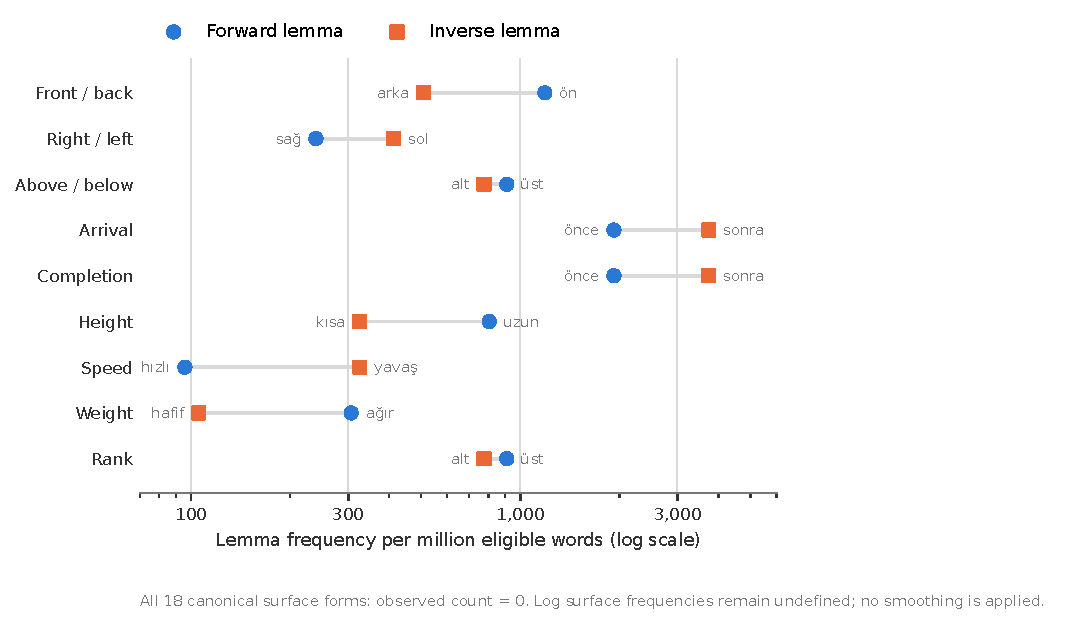
\includegraphics[width=\linewidth]{figures/manuscript/fig3_lemma_frequencies.pdf}
  \caption{Observed canonical surface counts and lemma frequency proxies for the nine forward/inverse
  relation pairs. Surface zeros are measured zeros; lemma counts are not sense-disambiguated counts of the
  full relation expression. Lines connect paired forward and inverse proxies; they are not confidence
  intervals. No model outcome is represented.}
  \label{fig:lemma}
\end{figure}

\begin{table}[t]
  \centering
  \caption{Independent relation-lemma counts in UD Turkish BOUN r2.18 (104,424 eligible lemma tokens).
  These are lemma counts, not sense-disambiguated relation frequencies. All 18 canonical surface-form counts
  are zero. Shared lemmas recur across templates.}
  \label{tab:lemma}
  \small
  \begin{tabular}{@{}llrlrr@{}}
    \toprule
    Relation & Forward lemma & Count & Inverse lemma & Count & $f_F/f_I$ \\
    \midrule
    Front / back  & ön    & 124 & arka  &  53 & 2.34 \\
    Right / left  & sağ   &  25 & sol   &  43 & 0.58 \\
    Above / below & üst   &  95 & alt   &  81 & 1.17 \\
    Arrival       & önce  & 201 & sonra & 390 & 0.52 \\
    Completion    & önce  & 201 & sonra & 390 & 0.52 \\
    Height        & uzun  &  84 & kısa  &  34 & 2.47 \\
    Speed         & hızlı &  10 & yavaş &  34 & 0.29 \\
    Weight        & ağır  &  32 & hafif &  11 & 2.91 \\
    Rank          & üst   &  95 & alt   &  81 & 1.17 \\
    \bottomrule
  \end{tabular}
\end{table}

\subsection{Tokenizer measurements}

The isolated-vocabulary export has 216 records: six registered configurations, nine relations, two
directions, and two languages. Counts cover the GPT-4o encoding configuration, the three Qwen
configurations, and the two Llama configurations. The Llama tokenizer assets are license-gated upstream;
they were vendored at the registered immutable revisions after license acceptance, with every file verified
against its upstream Git object hash, rather than being inferred from another tokenizer (an earlier retained
measurement records them as explicitly unavailable). A tokenizer measurement does not mean that model
weights were loaded or that its answers were evaluated.

All 216 isolated-vocabulary records are measured (Table~\ref{tab:tokenizers}). Across the 18 matched
relation-term pairs in each configuration, the median Turkish/English term-token ratio is 2.75 for
the GPT-4o encoding, 2.25 for each Qwen configuration, and 2.00 for each Llama configuration; observed
ratios across configurations range from 0.75 to 6. These are medians of matched ratios, not ratios of
median token counts. They summarize the selected lexical inventory without inferential confidence
intervals.

\begin{table}[t]
  \centering
  \caption{Tokenizer preprocessing coverage, not inference results. Each configuration has 18 Turkish and 18
  English relation terms; ratios use matched isolated terms. The three Qwen configurations yield identical
  term counts, as do the two Llama configurations; neither family contributes independent tokenization
  samples.}
  \label{tab:tokenizers}
  \small
  \begin{tabular}{@{}lrrrr@{}}
    \toprule
    Configuration & Measured & Median TR & Median EN & Median TR/EN \\
    \midrule
    GPT-4o / o200k\_base  & 36/36 & 4.0 & 2.0 & 2.75 \\
    Qwen2.5-0.5B / HF     & 36/36 & 5.0 & 2.5 & 2.25 \\
    Qwen2.5-1.5B / HF     & 36/36 & 5.0 & 2.5 & 2.25 \\
    Qwen2.5-1.5B / vLLM   & 36/36 & 5.0 & 2.5 & 2.25 \\
    Llama3.2-1B / HF      & 36/36 & 4.0 & 2.5 & 2.00 \\
    Llama3.2-3B / HF      & 36/36 & 4.0 & 2.5 & 2.00 \\
    \bottomrule
  \end{tabular}
\end{table}

\begin{figure}[t]
  \centering
  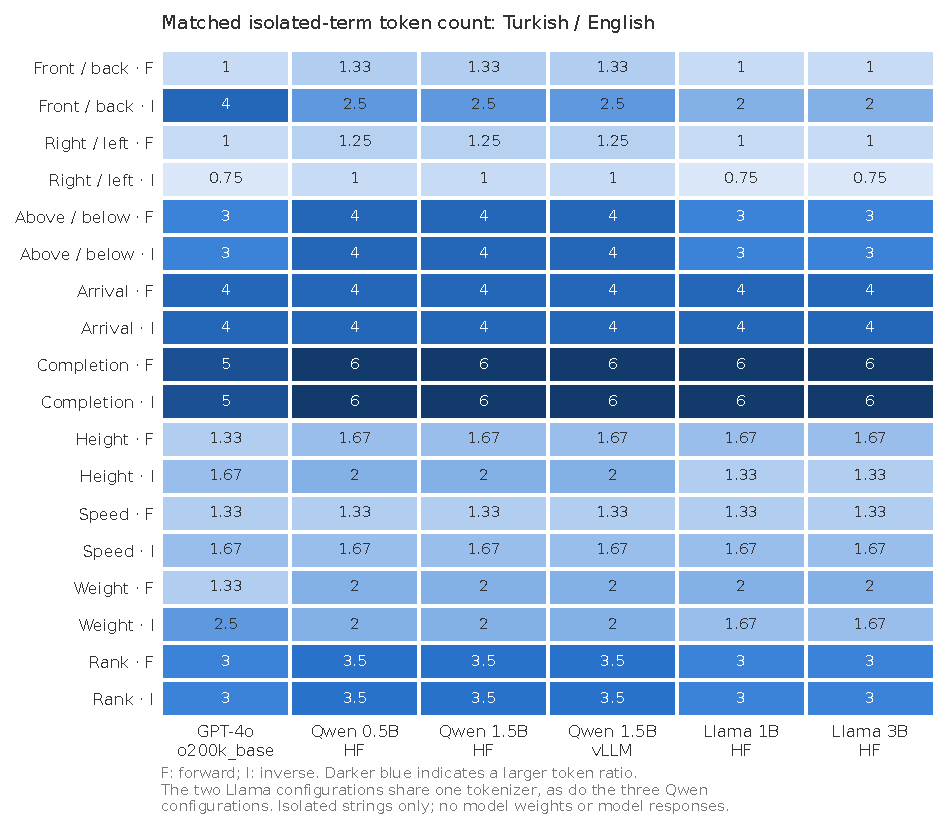
\includegraphics[width=0.94\linewidth]{figures/manuscript/fig4_token_ratios.pdf}
  \caption{Verified isolated relation-term tokenization. Matched Turkish/English measurements and
  forward/inverse differences describe the lexical strings and retained tokenizer assets; these are not
  model-performance comparisons.}
  \label{fig:tokens}
\end{figure}

Figure~\ref{fig:tokens} compares measured term tokenization across languages and directions on matched
lexical entries. Shared-tokenizer configurations are shown as configurations, not treated as independent
model families or independent replications. A ratio above one indicates a longer Turkish tokenization for
that lexical measurement and tokenizer. It does not imply a corresponding accuracy loss. Isolated
expressions, complete plain-text prompts, chat templates, and provider-billed usage have different scopes
\citep{rust2021tokenizer, ahia2023languages, petrov2023tokenizers}.

The corpus and tokenization audit provides features for RQ4; the executed pilot join
(Section~\ref{sec:pilot}) yields direction-specific diagnostics but cannot identify the
performance-association component from one relation family. The tokenized prompt preview is bounded to
$n = 4$; the isolated-term export should not be described as an analysis of full chat length across the
entire benchmark. Outcome analyses join by the exact latent/presentation coordinate and model/tokenizer
revision.

\subsection{What remains empirically unanswered}

Table~\ref{tab:availability} prevents preprocessing observations from being mistaken for answers to
RQ1--RQ5. The exploratory pilot evaluation of Section~\ref{sec:pilot} supplies the first genuine
accuracy-versus-$n$ curves, $R/D/U$ decompositions, and declared-family tests on the pilot split and one
relation family; the supplemental sweep of Section~\ref{sec:p1-local} extends them to all nine relation
families and four model scales; and the completed human review of Section~\ref{sec:review} backs the
sampled stimuli's grammaticality and meaning preservation. Confirmatory status still requires the
frozen-test design. The figures in the preceding subsections visualize actual construction/feature
measurements and a conceptual pipeline. No source-paper model scores are relabeled as Turkish-CBE results.

\begin{table}[t]
  \centering
  \caption{Outcome availability. NA is unavailable, not zero performance. ``Pilot (exploratory)'' denotes
  the executed pilot-split runs of Section~\ref{sec:pilot}; no confirmatory frozen-test estimate is
  reported.}
  \label{tab:availability}
  \small
  \begin{tabular}{@{}lp{0.47\linewidth}l@{}}
    \toprule
    Target & Required evidence & Current status \\
    \midrule
    Turkish--English gap        & Matched genuine answers and all-planned accuracy        & Pilot + sweep (exploratory) \\
    Morphosyntactic robustness  & Canonical/equivalent answers, $R/D/U$, coverage          & Pilot + sweep (exploratory) \\
    Complexity/distance profiles & Answers separated by $n$, $d$, and query type           & Pilot + sweep (exploratory) \\
    Lexical bias associations   & Direction-specific predictions joined to measured features & Pilot (diagnostics only) \\
    Stimulus linguistic validity & Two-reviewer sampled review with predeclared policy      & Completed (sampled) \\
    Reasoning/adaptation gains  & Matched intervention runs and recorded budgets           & Trained; evaluation gated \\
    \bottomrule
  \end{tabular}
\end{table}

\section{Exploratory Model Evaluation and Linguistic Validation}
\label{sec:pilot}

This section reports the genuine model outcomes obtained under the framework and their linguistic
validation, in chronological order: two complete registered pilot runs of 1,512 calls each, executed on
27 October 2026 on the pilot split (the first six subsections below); a supplemental quantized evaluation
of four open-weight scales over 16,618 matched prompts each (Section~\ref{sec:p1-local}); and the
subsequently completed two-reviewer Turkish linguistic review of 360 stimuli sampled from the same frozen
prompt population (Section~\ref{sec:review}). Every model result in this section is \emph{exploratory}: the
runs exercise the full execution and analysis machinery and motivate the confirmatory design, but the
execution-gate receipts for confirmatory authorization were not issued, no frozen-test evaluation has been
performed, and RQ1--RQ5 are not answered confirmatorily.

\subsection{Runs, shared cohort, and execution integrity}

Two registered model configurations were enabled by explicit user selection: Qwen2.5-0.5B-Instruct at a
pinned immutable revision, executed locally with greedy decoding (CPU, float32), and the dated snapshot
\texttt{gpt-4o-2024-08-06}, queried through its provider API at temperature zero. Both runs executed the
same immutable plan cohort: entity counts $n \in \{4, 8, 16, 32\}$ with eight latent orders per size,
endpoint, internal, and distance-controlled queries, the \texttt{spatial\_front} relation,
\texttt{native\_shared} names, English canonical and equivalent conditions, and all seven Turkish
conditions (canonical, general equivalent, and P1--P5). Each of the nine language/presentation conditions
contains the same 168 planned queries; prompts are byte-identical across models.

\begin{table}[t]
  \centering
  \caption{Executed pilot runs. Both runs completed all planned calls with zero invalid and zero
  wrong-language answers under the strict parser.}
  \label{tab:pilotruns}
  \small
  \begin{tabular}{@{}llrr@{}}
    \toprule
    Model & Execution & Calls & Invalid \\
    \midrule
    Qwen2.5-0.5B-Instruct & local, greedy, CPU/float32 & 1\,512/1\,512 & 0 \\
    gpt-4o-2024-08-06     & provider API, temperature 0 & 1\,512/1\,512 & 0 \\
    \bottomrule
  \end{tabular}
\end{table}

The registered pilot runs followed the recorded inference, provenance, and recovery procedures in full
(the supplemental quantized evaluation of Section~\ref{sec:p1-local} is a separately labeled exploratory
experiment that reuses the frozen prompts and parser without claiming completion of the prospective
confirmatory execution gates): write-once plans re-derived and byte-compared
at execution time, append-only raw request/response records with full lineage, and checkpointed resumption.
One transient transport error occurred in the API run; following the ambiguity policy, the run halted and
resumed only after an explicit, logged retry resolution acknowledging duplicate risk. Two earlier API run
identifiers are retained as provenance of failed attempts (a local TLS misconfiguration before any billable
call, and a provider spending-limit refusal with zero billed generations); neither contributes records to
the analyzed run.

\subsection{A degenerate responder: perfect invariance without competence}

Qwen2.5-0.5B-Instruct emitted a constant answer per language on all 1,512 prompts: affirmative
(\emph{YES}) on every English prompt and negative (\emph{HAYIR}) on every Turkish prompt, at every size,
query type, and presentation. Because planned gold labels are balanced, marginal accuracy is exactly 0.500
in every stratum and the paired Turkish--English difference is zero everywhere. Raw invariance is perfect:
$\widehat{I} = 1$ within each language, with $\widehat{R} = \widehat{D} = 0.5$ and $\widehat{U} = 0$.
The pooled answer rate is degenerate ($q \in \{0, 1\}$), so $I_e = 1$ and $\kappa_{\mathrm{CBE}}$ is
undefined with the recorded reason \texttt{constant\_pooled\_answer}, exactly as
Equation~\eqref{eq:kappa} prescribes.

This run is a concrete demonstration of the framework's central measurement argument rather than a mere
null result. An evaluation reporting raw cross-presentation agreement would have scored this model as
perfectly robust; the joint presentation of $R$, $D$, $U$, and the chance correction instead identifies a
responder whose ``consistency'' consists entirely of shared correct-by-chance and shared wrong answers.
No competence claim, positive or negative, beyond this behavioral characterization is made for the model.

\subsection{GPT-4o: graded competence and a presentation cliff}

All 1,512 GPT-4o answers were valid and in the requested language, so all-planned and valid-pair
denominators coincide and valid-pair coverage is 1 in every stratum below. Figure~\ref{fig:pilot}
summarizes the marginal structure. Pooled all-planned accuracy is 72.0\% on English ($N = 336$) and
57.8\% on Turkish ($N = 1{,}176$). The two English conditions agree closely (canonical 71.4\%, equivalent
72.6\%), while the Turkish conditions separate: canonical 67.9\% and P1 68.5\% at the top; equivalent
57.7\%, P2 58.3\%, P4 61.9\%, and P5 53.6\% in between; and P3, the alternative constituent construction,
at 36.9\% --- below the 50\% balanced baseline.

\begin{figure}[t]
  \centering
  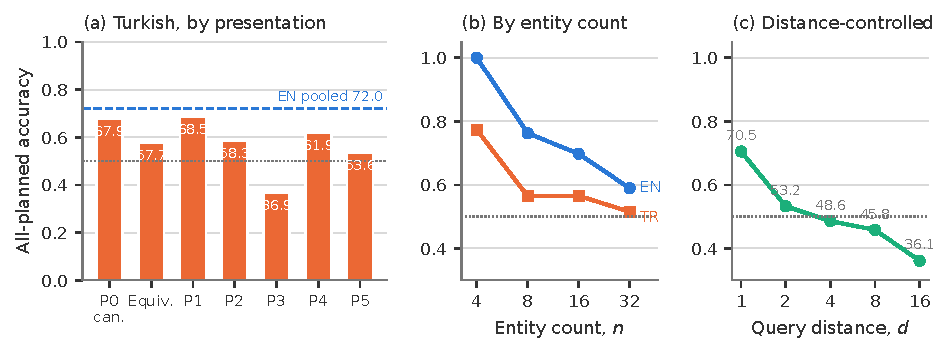
\includegraphics[width=\linewidth]{figures/manuscript/fig5_pilot_gpt4o.pdf}
  \caption{Exploratory pilot accuracy of \texttt{gpt-4o-2024-08-06} (all answers valid; all-planned
  accuracy; dotted line: 50\% balanced baseline). (a) Turkish accuracy by presentation condition with the
  pooled English reference; 168 prompts per condition. (b) Accuracy by entity count and language.
  (c) Pooled accuracy of distance-controlled queries by latent query distance $d$; per-distance counts
  vary by design (288, 216, 216, 144, and 72 prompts). Pilot split, one relation family, stimulus review
  in Section~\ref{sec:review}; these curves are not confirmatory answers to RQ1--RQ3.}
  \label{fig:pilot}
\end{figure}

Accuracy declines monotonically with entity count in both languages (English $100\% \to 58.9\%$ and
Turkish $77.4\% \to 51.5\%$ from $n = 4$ to $n = 32$) and with latent query distance within the
distance-controlled stratum ($70.5\%$ at $d = 1$ to $36.1\%$ at $d = 16$). The pooled query-type ordering
is endpoint $76.4\%$ $>$ internal $64.9\%$ $>$ distance-controlled $55.0\%$. Sustained below-baseline
accuracy at large $d$ indicates a systematic directional error rather than random guessing. Predicted
answer rates also differ by language: the affirmative rate is 0.476 on English but 0.680 on Turkish
against balanced gold labels, i.e.\ Turkish errors skew toward \emph{EVET}.

\begin{table}[t]
  \centering
  \caption{Pooled descriptive paired profiles for GPT-4o (168 jointly valid pairs per row; valid-pair
  coverage 1.0, so Equations~\eqref{eq:identities}--\eqref{eq:strict} coincide with their all-planned
  counterparts). $q$ is the pooled affirmative rate of Equation~\eqref{eq:kappa}. Pooling crosses size and
  query-type strata, so these values are summaries of the executed cohort, not stratum estimands;
  per-stratum profiles with cluster-bootstrap intervals are in the released analysis tables.}
  \label{tab:pilotprofiles}
  \small
  \begin{tabular}{@{}lccccc@{}}
    \toprule
    Comparison & $R$ & $D$ & $U$ & $q$ & $\kappa_{\mathrm{CBE}}$ \\
    \midrule
    TR canonical $\to$ TR equivalent & 0.458 & 0.202 & 0.339 & 0.652 & 0.253 \\
    TR canonical $\to$ TR P1         & 0.565 & 0.202 & 0.232 & 0.640 & 0.496 \\
    TR canonical $\to$ TR P2         & 0.500 & 0.238 & 0.262 & 0.667 & 0.411 \\
    TR canonical $\to$ TR P3         & 0.298 & 0.250 & 0.452 & 0.673 & $-0.027$ \\
    TR canonical $\to$ TR P4         & 0.542 & 0.244 & 0.214 & 0.631 & 0.540 \\
    TR canonical $\to$ TR P5         & 0.446 & 0.232 & 0.321 & 0.667 & 0.277 \\
    EN canonical $\to$ TR canonical  & 0.565 & 0.173 & 0.262 & 0.560 & 0.469 \\
    EN equivalent $\to$ TR equivalent & 0.476 & 0.173 & 0.351 & 0.568 & 0.284 \\
    \bottomrule
  \end{tabular}
\end{table}

Table~\ref{tab:pilotprofiles} gives the pooled paired decomposition. The P3 contrast is qualitatively
different from every other Turkish perturbation: robust correctness falls to $\widehat{R} = 0.298$,
presentation dependence rises to $\widehat{U} = 0.452$, and the pooled chance-corrected agreement is
approximately zero ($\kappa_{\mathrm{CBE}} = -0.027$): the canonical and P3 responses exhibit little
agreement beyond the specified pooled-marginal reference, despite being generated from identical latent
reasoning problems. Consistent with Section~\ref{sec:statistics}, this does not establish stochastic
independence or identify an internal mechanism. The cross-language rows show the second
mechanism the decomposition separates: moving from English to Turkish converts correct answers into
presentation-dependent ones ($U$ up to 0.351) rather than into shared errors ($D$ stable at 0.173).

\subsection{Inferential results at pilot power}

Declared-family inference behaves as the design anticipates at this scale. Across the 70 matched
Turkish--English strata, the accuracy difference is negative in 31 and positive in 10 (mean $-0.098$), but
no individual eight-pair stratum survives Holm correction: the direction is consistent while per-stratum
McNemar tests are underpowered, which is precisely the regime the frozen-test sample sizes were chosen to
escape. The P3 effect, by contrast, is strong enough to register even here: the canonical-versus-P3
family contains the only Holm-surviving strata in the study (two strata at $n = 32$, endpoint and
distance-controlled, each with difference $-0.75$ and Holm-adjusted $p = 0.031$). Cluster-bootstrap
intervals accompany every reported stratum in the released tables; pooled values above are descriptive.

\subsection{Exploratory lexical-direction diagnostics (RQ4)}

The retained lexical pipeline was additionally executed joined to both completed runs, producing the
declared answer-share diagnostics, lexical-direction profiles, Spearman associations, and controlled
regression specifications on the pilot observations. Its most interpretable output is a pronounced
\emph{direction asymmetry} in GPT-4o (Table~\ref{tab:direction}): against balanced gold labels, queries
asked with the inverse predicate (Turkish \emph{arkasındadır}, English \emph{behind}) are answered
affirmatively far more often and less accurately than forward queries (\emph{önündedir} / \emph{in front
of}). The asymmetry appears in both languages and is largest in Turkish, where the inverse-direction
affirmative share reaches 0.793; it accounts for most of the pooled Turkish affirmative bias reported
above. The predeclared response-tendency diagnostic flags Qwen2.5-0.5B in every stratum (excessive
\emph{no} in Turkish, excessive \emph{yes} in English), while GPT-4o pools within thresholds overall and
crosses the affirmative threshold only in inverse-direction Turkish strata.

\begin{table}[t]
  \centering
  \caption{Direction-specific pilot diagnostics for GPT-4o (all planned gold labels balanced at 0.500;
  all answers valid). Forward queries use \emph{önündedir} / \emph{in front of}; inverse queries use
  \emph{arkasındadır} / \emph{behind}. These are descriptive shares on one relation family; direction
  changes the lexical predicate, the construction, and tokenization together, so no single cause is
  identified.}
  \label{tab:direction}
  \small
  \begin{tabular}{@{}llrcc@{}}
    \toprule
    Language & Query direction & $N$ & Accuracy & Affirmative share \\
    \midrule
    Turkish & forward & 588 & 0.639 & 0.568 \\
    Turkish & inverse & 588 & 0.517 & 0.793 \\
    English & forward & 168 & 0.768 & 0.399 \\
    English & inverse & 168 & 0.673 & 0.554 \\
    \bottomrule
  \end{tabular}
\end{table}

This asymmetry aligns suggestively with the preprocessing measurements: the forward lemma \emph{ön} is
more than twice as frequent as the inverse lemma \emph{arka} in the retained corpus measurement
(Table~\ref{tab:lemma}), and for the GPT-4o encoding the inverse Turkish predicate is four times its
English counterpart's token length while the forward pair is matched (Figure~\ref{fig:tokens}). The
design, however, cannot promote this alignment to an association: the pilot cohort contains a single
relation family, so each correlation cell holds at most two lexical units, and the retained Spearman and
regression outputs record exactly that --- the large majority of cells return \texttt{constant\_input},
\texttt{insufficient\_pairs}, \texttt{insufficient\_rows}, or \texttt{rank\_deficient} rather than a
coefficient, as the protocol requires of unsupported or collinear fits. RQ4's association component
therefore remains unanswered; answering it requires the multi-relation frozen design, where the nine
relation families provide the cross-vocabulary variation this cohort lacks.

\subsection{Training backend execution (RQ5)}

The optional adaptation backend was executed for the first time on rented CUDA hardware (RTX 6000 Ada,
48\,GB, bf16) under the configuration's declared dependency pins, which this run validates. All five
training arms of the pilot profile --- LoRA SFT, paired SFT, SFT with the JS consistency term, and both
GRPO objectives --- completed on Qwen2.5-1.5B-Instruct from a hash-verified local weights bundle, with
immutable plans, zero gate blockers, recorded hardware and token budgets, and deterministic seeding. The
pilot profile is smoke-scale by design (two optimizer steps per arm), so these runs validate the training
machinery and its accounting, not any adaptation effect. Both GRPO arms recorded one zero-gradient step,
the exact diagnostic the plan's warnings predict for binary prompt-normalized advantages. The matched
base-versus-adapter evaluation remains unexecuted: the protocol's evaluation design is frozen at nine
sizes on the test split (10,224 calls per arm), which requires a dataset-bound execution-gate review
receipt that has not been issued (the completed stimulus review of Section~\ref{sec:review} is a separate
instrument); no reduced evaluation is expressible within the validated configuration, deliberately. RQ5
therefore remains empirically unanswered, with trained adapters retained should that receipt be produced.

\subsection{Supplemental quantized local evaluation: an open-weights scale sweep}
\label{sec:p1-local}

To test whether the pilot's findings are idiosyncrasies of one proprietary model, the frozen protocol was
additionally executed across the Qwen2.5 instruction-tuned family at four scales (0.5B, 3B, 7B, 14B) in a
\emph{supplemental quantized local arm}: Q4\_K\_M GGUF weights served by Ollama (weight digests recorded
per run), greedy decoding at temperature 0 with fixed seed, the audited message constructor with run-time
prompt-hash re-verification, and the registered strict parser. Because quantized weights are not the
registered fp/bf16 snapshots, this arm is labeled on every record and is never pooled with
registered-provider results; agreement across arms is read as qualitative replication, not equivalence.
The expanded manifest holds 16{,}618 prompt identities drawn exclusively from the pilot split (all nine
relation families, sizes $4 \le n \le 128$, balanced paired sampling across languages, presentations, and
naming controls; the frozen test sizes remain untouched), and every prompt passed an automated semantic
validation of its stated facts and gold label before execution. All four arms answered all 16{,}618
prompts with zero transport failures; unparseable responses (0, 25, 184, and 247 from 0.5B to 14B, the
latter coinciding with output-length truncation) are retained and scored as errors under the all-planned
estimand. Like the pilot, this expanded run exceeds the predeclared human-review threshold; the stimulus
review of Section~\ref{sec:review} was subsequently completed on this run's prompt population, but no
execution-gate receipt was issued, and the arm remains exploratory (quantized weights, pilot split).

\begin{figure}[t]
  \centering
  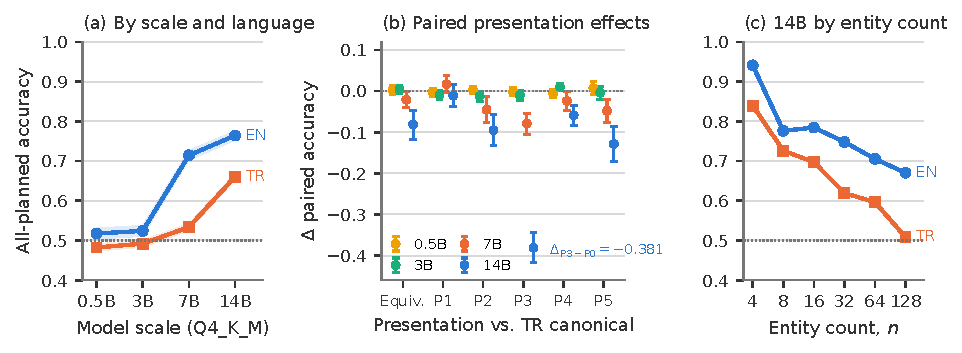
\includegraphics[width=\linewidth]{figures/manuscript/fig6_p1_quantized_scaling_annotated.pdf}
  \caption{Supplemental quantized local evaluation of the Qwen2.5 instruct family (Q4\_K\_M; all-planned
  accuracy over 16{,}618 prompts per model; dotted lines: 50\% balanced baseline and zero effect).
  (a) Accuracy by model scale and language with Wilson bands. (b) Query-matched paired accuracy
  difference of each Turkish presentation minus the Turkish canonical form (negative = reduction), with
  latent-cluster bootstrap 95\% intervals and the dotted zero-effect reference; the annotated point is the
  14B P3 effect ($\Delta_{\mathrm{P3-P0}} = -0.381$, 95\% CI $[-0.418, -0.344]$). Pooled single-condition
  accuracies are compositionally confounded and are not shown.
  (c) Accuracy by entity count for the 14B model. Pilot split, quantized supplemental arm, stimulus
  review in Section~\ref{sec:review}; not confirmatory answers to RQ1--RQ3.}
  \label{fig:p1scaling}
\end{figure}

The sweep reproduces both pilot regimes, and the evaluated scales suggest a transition from predominantly
response-biased behavior in the smaller models toward more discriminative performance at 7B and 14B
(Figure~\ref{fig:p1scaling}a); with four evaluated sizes of one quantized family, no precise or universal
scaling threshold is identified. The 0.5B and 3B models are near-constant responders --- 0.5B answers
\emph{hay\i{}r} on 95.8\% of Turkish and \emph{yes} on 99.8\% of English calls, and its paired
English--Turkish profile is the degenerate signature in pure form ($R = 0.017$, $U = 0.970$: on almost
every matched pair exactly one language is ``correct'' because the two constant answers disagree).
Discrimination emerges at 7B in English only (71.4\% vs.\ 53.4\%; paired gap $-0.176$, cluster-bootstrap
95\% CI $[-0.241, -0.106]$) and reaches both languages at 14B (76.4\% vs.\ 66.1\%; paired gap $-0.075$,
CI $[-0.126, -0.020]$). Because pooled pairs share latent orders, conventional row-level McNemar inference
is not appropriate for these dependent observations; uncertainty for all language and presentation
contrasts is therefore estimated by latent-order cluster bootstrapping, and the intervals are labeled
exploratory.

Two pilot findings replicate in open weights and sharpen with scale. First, the P3 presentation cliff:
on query-matched pairs the P3-minus-canonical accuracy difference for the 14B model is
$\widehat{\Delta}_{\mathrm{P3-P0}} = -0.381$ (95\% cluster-bootstrap CI $[-0.418, -0.344]$; 554 vs.\ 40
discordant pairs), a reduction of 38.1 percentage points that drops P3 accuracy to 43.1\% --- below the
balanced baseline --- while the same contrast at 7B is already credible at $-0.079$ and absent in the
constant responders (Figure~\ref{fig:p1scaling}b). Per-stratum agreement decays with complexity
($\kappa_{\mathrm{CBE}}$ for canonical-versus-equivalent at 14B: $0.57$ at $n{=}4$ to $0.12$ at
$n{=}128$), and for canonical-versus-P3 it turns negative at $n{=}16$ and $n{=}32$: systematic answer
flips, not noise. Second, the complexity decay: 14B Turkish accuracy falls monotonically from 83.9\% at
$n{=}4$ to 50.8\% --- chance --- at $n{=}128$ (English 94.1\% to 67.0\%; Figure~\ref{fig:p1scaling}c),
mirroring the GPT-4o pilot curve. The naming family, whose pairs are cluster-unique and therefore admit
exact inference, adds one Holm-surviving result: at 14B, replacing native Turkish entity names with shared
symbolic labels costs $11.7$ points (McNemar $b{=}59$, $c{=}24$, Holm-adjusted $p = 3.8\times10^{-4}$),
while English transliteration of the same names costs nothing measurable --- once competence exists,
entity-name surface form matters, and the deficit is not explained by transliteration alone.

\subsection{Completed two-reviewer Turkish linguistic review}
\label{sec:review}

The human review that the construction audit required was executed by two independent Turkish-proficient
reviewers on a 360-item stratified sample drawn from the frozen pilot-split prompts (all nine relation
families, every Turkish presentation, P3 deliberately oversampled at 144 items; annotation protocol,
blinding, and the inclusion policy were fixed before any judgment was entered). Each reviewer
independently rated grammaticality and naturalness (1--5), semantic equivalence of each transformed
prompt against its canonical counterpart, and clause-level ambiguity. The predeclared policy admits a
transformed item to confirmatory analysis only when both reviewers rate grammaticality $\ge 4$ and agree
the transformation is meaning-preserving.

The outcome is sharply structured. Semantic equivalence is unanimous: both reviewers judged all 324
transformed items meaning-preserving, and no item was flagged ambiguous. Grammaticality excluded exactly
one construction: the P3 realization of \emph{temporal\_completion}, whose 16 sampled items one reviewer
rated ungrammatical (grammaticality 2, ``devrik c\"umle yap\i{}s\i{}''), leaving 344 of 360 items
confirmatory-eligible. Naturalness --- which the policy deliberately records but does not gate on --- is
the one contested dimension: exact inter-reviewer agreement is low (33\%, Cohen's $\kappa = 0.06$), the
two reviewers' P3 naturalness medians are 4 versus 2, and only 6 of 144 P3 items received $\ge 4$ from
both. (Chance-corrected agreement is degenerate for grammaticality and ambiguity because one or both
reviewers used a single category almost everywhere; raw agreement is 96\% and 100\%.)

The review therefore narrows, but does not fully close, the stimulus-artifact explanation of the P3
cliff. A review-driven sensitivity reanalysis removes the excluded relation entirely from the P3
contrast: the 14B query-matched deficit survives unchanged or deepens ($-0.381$ over all nine relations
versus $-0.408$, cluster-bootstrap 95\% CI $[-0.446, -0.370]$, with \emph{temporal\_completion} removed;
the 7B contrast is unchanged at $-0.080$). The P3 collapse is thus measured on stimuli that two
independent reviewers unanimously certify as meaning-preserving and (outside one excluded construction)
grammatical, while their discourse naturalness remains contested --- the honest residual reading is that
models fail on grammatical, truth-preserving but discourse-atypical constituent orders, a regime in which
a competent human reader does not lose the ability to evaluate the stated facts. Review artifacts,
per-item decisions, and agreement statistics are released with the framework
(\texttt{validation/review\_results/}); the separate execution-gate receipts for runs above the declared
call threshold were not issued, so no evaluation in this manuscript claims confirmatory status.

\subsection{What this evaluation does and does not establish}

These experiments establish that the end-to-end protocol --- immutable planning, gated execution, strict
parsing, paired analysis with declared denominators, and multiplicity control --- runs unmodified on local,
provider-hosted, and quantized local models, and that the paired decomposition discriminates in practice
between degenerate constant responders and models with graded, presentation-sensitive competence, with the
same qualitative structure recurring from the registered pilot to the digest-pinned nine-relation sweep.
They do not establish a confirmed Turkish--English gap, a morphology effect, or a complexity law:
everything remains on the pilot split; strata share latent orders; and the supplemental arm is quantized
and therefore not precision-comparable to registered snapshots. Section~\ref{sec:discussion} synthesizes
the findings and their interpretive boundaries, including what the completed review does and does not
resolve about P3. These results size and motivate, but do not replace, the preregistered frozen-test
evaluation.

\section{Discussion}
\label{sec:discussion}

Table~\ref{tab:findings} consolidates the main empirical findings of Section~\ref{sec:pilot}; the
subsections below synthesize what they establish and where their interpretive boundaries lie. All findings are exploratory and describe the evaluated models, cohorts, and settings.

\begin{table}[t]
  \centering
  \caption{Consolidated exploratory findings. ``Sweep'' denotes the supplemental quantized Qwen2.5
  evaluation (16,618 matched prompts per model, pilot split, all nine relation families); paired effects
  are query-matched signed differences (condition minus canonical, or Turkish minus English) with
  latent-cluster bootstrap 95\% intervals; negative values are reductions. pp = percentage points.}
  \label{tab:findings}
  \small
  \setlength{\tabcolsep}{4.5pt}
  \begin{tabular}{@{}p{0.105\linewidth}p{0.29\linewidth}p{0.295\linewidth}p{0.175\linewidth}@{}}
    \toprule
    Dimension & Main observation & Supporting evidence & Interpretation \\
    \midrule
    Model scale & All-planned accuracy rises from chance to 69.2\% across 0.5B--14B &
      Sweep: 49.3\%, 50.2\%, 58.7\%, 69.2\% (Fig.~\ref{fig:p1scaling}a) &
      Scale-associated discrimination in the evaluated family \\
    Language & English accuracy exceeds Turkish once models discriminate &
      14B matched canonical pairs: 78.2\% vs.\ 70.7\%, paired gap $-7.5$\,pp [$-12.6$, $-2.0$]
      (all-condition marginals 76.4\%/66.1\%); 7B: $-17.6$\,pp [$-24.1$, $-10.6$] &
      Language-dependent behavior on matched problems \\
    Presentation & P3 constituent order produces a large accuracy decrease &
      14B: $-38.1$\,pp [$-41.8$, $-34.4$], discordant 554 vs.\ 40; $-40.8$\,pp [$-44.6$, $-37.0$] after
      the review exclusion & Constituent-order sensitivity on meaning-preserving input \\
    Complexity & Accuracy decreases monotonically with entity count &
      14B Turkish: 83.9\% at $n{=}4$ to 50.8\% at $n{=}128$ (Fig.~\ref{fig:p1scaling}c) &
      Input-size sensitivity \\
    Naming & Shared symbolic labels reduce accuracy at 14B &
      $-11.7$\,pp, McNemar $b{=}59$, $c{=}24$, Holm $p = 3.8\times10^{-4}$ &
      Entity-representation sensitivity \\
    Invariance & Constant responders show near-perfect within-language invariance at chance accuracy &
      Pilot 0.5B: $I = 1.00$ across presentations, $\kappa_{\mathrm{CBE}}$ undefined; sweep 0.5B TR
      canonical vs.\ equivalent: $I = 0.96$ & Raw invariance does not establish correctness \\
    Response bias & Language-conditioned constant answers produce cross-language disagreement &
      Sweep 0.5B EN--TR pairs: $R = 0.017$, $U = 0.970$ (constant \emph{yes} in EN, \emph{hay\i{}r} in TR)
      & Deterministic bias, not instability, drives the disagreement \\
    \bottomrule
  \end{tabular}
\end{table}

\subsection{Correctness and presentation invariance are distinct}

The paired decomposition supports questions that a marginal accuracy table cannot answer. A small average
difference between canonical and equivalent prompts can coexist with large, offsetting correct-to-wrong and
wrong-to-correct flows; conversely, agreement can improve because a model repeats a wrong label.
Equations~\eqref{eq:identities}--\eqref{eq:strict} specify the evidence needed to distinguish these cases:
shared-valid $R/D/U$, all-planned accuracy and strict $R$, invalid rates, and coverage. The evaluated models
realize both failure modes, and the constant responders illustrate two complementary observations that
must not be conflated. Within a language, a near-constant responder is almost perfectly invariant without
any competence: the registered pilot 0.5B run attains $I = 1.00$ across Turkish presentations at chance
accuracy with $\kappa_{\mathrm{CBE}}$ undefined, and the sweep 0.5B (Turkish \emph{hay\i{}r} on 95.8\% of
Turkish calls, \emph{yes} on 99.8\% of English calls) still reaches $I = 0.96$ on canonical-versus-equivalent
pairs. Across languages, the same deterministic behavior produces the opposite signature: on
English--Turkish pairs $R = 0.017$ with $U = 0.970$, because the two language-conditioned constant answers
disagree and exactly one side is scored correct on almost every pair --- language-conditioned response
bias, not response instability. Any protocol that reported within-language agreement without the
decomposition would have certified this model. The chance correction
has a correspondingly limited role: constant outputs make $\kappa_{\mathrm{CBE}}$ undefined by construction,
and its pooled-marginal baseline discounts one particular independent-answer bias reference without
modeling failure causally or proving stochastic independence. Correctness and invariance remain behavioral
properties; explanation text adds an observation channel, not access to the model's internal computation
\citep{turpin2023unfaithful}.

\subsection{Turkish constituent-order sensitivity}

The P3 result is the sharpest finding. On query-matched pairs, the P3-minus-canonical accuracy difference
for the 14B model is $-0.381$ (95\% CI $[-0.418, -0.344]$; 554 vs.\ 40 discordant pairs) --- a reduction of
38.1 percentage points that takes Turkish P3 accuracy below the balanced baseline --- with a credible
$-0.079$ precursor already at 7B and no effect in the constant responders; the registered pilot found the
same collapse in GPT-4o (36.9\% under P3). The completed review (Section~\ref{sec:review}) bounds its interpretation from both
sides. On one side, both reviewers unanimously judged the sampled transformations meaning-preserving, and
the one construction that failed grammaticality for one reviewer (\emph{temporal\_completion} under P3) is
removed by a sensitivity reanalysis in which the effect persists and deepens ($-0.408$, 95\% CI
$[-0.446, -0.370]$). A pure stimulus-grammaticality artifact is therefore ruled out for the retained
constructions. On the other side, the reviewers' naturalness judgments genuinely differ (P3 medians 4
vs.\ 2), so the transformations cannot be claimed uniformly natural in every discourse context; this
documented linguistic variation qualifies, but does not invalidate, the finding. The supported conclusion
is that the evaluated models exhibit substantial behavioral sensitivity to meaning-preserving Turkish
constituent-order variation, including constructions both human reviewers accepted as grammatical. The
effect does not by itself identify \emph{which} capacity fails---logical inference, syntactic parsing, or
the representation of discourse-atypical input---and the review, which measured linguistic judgments
rather than human task accuracy, does not license a comparison with human reasoning performance on the
same prompts.

\subsection{Model scale and multilingual reasoning}

The evaluated Qwen2.5 family progresses from strongly biased, near-constant response behavior (0.5B, 3B)
toward discriminative performance, in English before Turkish (7B: 71.4\% vs.\ 53.4\%) and then in both
(14B: 76.4\% vs.\ 66.1\%). Scale is associated with higher accuracy, a narrower but persistent language
gap, and---critically---\emph{increasing} absolute presentation sensitivity: the P3 deficit grows from
nothing (constant responders) through $-7.9$\,pp (7B) to $-38.1$\,pp (14B), and per-stratum
$\kappa_{\mathrm{CBE}}$ for canonical-versus-equivalent decays with complexity at 14B (0.57 at $n{=}4$ to
0.12 at $n{=}128$). Improved canonical accuracy therefore does not guarantee equivalent robustness across
alternative linguistic presentations: the most capable evaluated model is simultaneously the most
presentation-sensitive in absolute terms. We do not claim that 7B marks a universal emergence threshold,
that parameter count is the sole causal factor, or that the pattern extends beyond this family; the
supplemental experiments use quantized weights from a single model lineage, and response bias, instruction
tuning, and training data co-vary with scale.

\subsection{Complexity and entity representation}

The endpoint shortcut makes a strong endpoint score ambiguous as evidence of transitive reasoning;
internal and distance-controlled questions reduce that specific shortcut without eliminating every
efficient strategy. Within those boundaries, the exploratory profiles are consistent: accuracy declines
monotonically with entity count in every discriminating model (14B Turkish reaches chance at $n{=}128$),
the pilot's endpoint $>$ internal $>$ distance-controlled ordering matches the shortcut analysis, and
below-baseline accuracy at large query distance indicates a systematic directional error rather than noise.
Changes with $n$ may still reflect retrieval, distraction, context length, or the distribution of queried
distances. Entity representation matters independently: replacing native Turkish names with shared symbolic
labels costs the 14B model 11.7 points (the only Holm-surviving McNemar result in the sweep), while English
transliteration of the same names costs nothing measurable---so the deficit is not explained by
transliteration alone. The pilot's direction asymmetry (Table~\ref{tab:direction}) aligns suggestively with
measured frequency and tokenization asymmetries, but the single-relation cohort leaves every lexical
association formally unidentified, and the retained specifications record refusals rather than
coefficients, exactly as the protocol requires.

\subsection{Implications for multilingual benchmark design}

These findings argue that multilingual reasoning benchmarks should report matched correctness and
presentation stability rather than accuracy alone. An accuracy-only leaderboard would have ranked the
constant responders near chance---correctly---but would also have certified their perfect cross-presentation
agreement had invariance been reported without correctness, and it would have missed that the strongest
evaluated model loses more than a third of its paired accuracy under one meaning-preserving Turkish
construction. Matching latent instances across languages, holding answers fixed under transformation,
declaring denominators, and separating $R$, $D$, and $U$ are each individually simple; their combination is
what makes the failure modes visible. The same structure also disciplines interpretation: measured zeros in
corpus frequency, tokenization ratios, and naturalness disagreement are reported as measured properties
with explicit scopes, not converted into causal explanations \citep{rust2021tokenizer, ahia2023languages,
petrov2023tokenizers}.

\subsection{Scope of the empirical evidence}

All model results are exploratory: pilot-split cohorts, one quantized model family in the sweep, no issued
execution-gate receipts, and no frozen-test evaluation. The framework's inferential machinery was sized for
the frozen test, and the pilot vindicates that sizing in both directions---eight-pair strata detect nothing
for the consistently negative Turkish--English contrast, while the P3 effect survives Holm correction even
at pilot scale. Null, adverse, or non-replicating confirmatory outcomes remain possible and would be
incorporated without changing definitions after observing results; Section~\ref{sec:limitations} records
the limitations and Section~\ref{sec:future} the confirmatory agenda.

\section{Limitations and Future Work}
\label{sec:limitations}

\subsection{Limitations of the present study}

\paragraph{Exploratory scope.}
All model evidence is exploratory and comes from the pilot split: the two registered pilot runs
(one relation family, one name control, $n \le 32$) and the supplemental sweep (nine relation families,
$n \le 128$) with quantized Q4\_K\_M weights that are not precision-comparable to registered fp/bf16
snapshots. The sweep covers a single model lineage (Qwen2.5 instruct), so model-family diversity is
limited; GPT-4o adds one proprietary configuration on the narrower pilot cohort. No confirmatory
frozen-test estimate exists, and no adaptation improvement has been evaluated---the executed training runs
are smoke-scale backend validation only.

\paragraph{Linguistic coverage and validation.}
The renderer covers a closed grammar and a finite relation and presentation inventory; Turkish morphology
and word order are richer than the implemented templates, and P4/P5 do not identify a pure morphology
manipulation. Shared generation/parsing code can conceal a common-mode mistake. The completed human review
(Section~\ref{sec:review}) found unanimous semantic-equivalence judgments and, outside one excluded
construction, acceptable grammaticality within the reviewed sample, but it is sampled rather than
exhaustive, and its naturalness dimension shows low inter-reviewer agreement; it certifies neither every
generated realization nor that every transformation is natural in every discourse context. Minimal-pair results in prior literature cannot validate our stimuli automatically.

\paragraph{Task and dependence structure.}
Strict total orders exclude partial orders, contradictory premises, ties, and open-world uncertainty.
Renamed orders are structurally isomorphic. Multiple queries, names, relations, and presentations share
each latent source, so prompt counts overstate independent sample sizes by orders of magnitude; all
inference in this article clusters on latent orders, and exact split separation does not establish absence
of pretraining contamination.

\paragraph{Frequency and tokenization proxies.}
BOUN has finite genre and sense coverage; surface $n$-gram and lemma opportunities differ; exact canonical
zeros need not reflect general usage; and lemma counts are not relation-sense counts. Tokenizer
measurements cover six registered configurations, with shared-tokenizer configurations not independent.
Isolated-string measurements exclude chat overhead and billed usage. With one relation family in the pilot
join, no lexical association is identified.

\paragraph{Inference and missingness.}
Context overflow, wrong-language answers, truncation, and provider nondeterminism may be systematically
associated with difficult items; conditional CBE statistics therefore always carry coverage and
all-planned counterparts. Cluster-bootstrap intervals depend on sufficient independent latent orders, and
the declared Holm families do not provide study-wide simultaneous error control. Where pooled pairs share
latent clusters, conventional row-level McNemar inference is not appropriate for the dependent
observations, and uncertainty is instead estimated by exploratory latent-order cluster-bootstrap
contrasts.

\subsection{Future work}
\label{sec:future}

The confirmatory agenda is specified and frozen but unexecuted. It comprises: (1) the preregistered
frozen-test evaluation under the declared primary families (test split, sizes up to $n = 1024$);
(2) the formal execution-gate approvals---dataset-bound two-reviewer receipts and pilot approval---that
authorize runs above the declared call threshold, which are future methodological procedures rather than
requirements of the present exploratory study; (3) additional model-family comparisons beyond Qwen2.5,
including full-precision registered snapshots; (4) the matched base-versus-adapter evaluation of the five
already-trained arms under the frozen 10,224-call-per-arm design; (5) reasoning-prompting interventions
under the declared budget and faithfulness caveats; (6) expanded linguistic and relation-family coverage,
including naturalness-controlled constituent-order stimuli that could close the residual P3 ambiguity; and
(7) multi-relation lexical-familiarity and tokenization analyses, which become identifiable once the
frozen design supplies cross-vocabulary variation.

\section{Conclusion}

Turkish-CBE contributes, first, a controlled bilingual reasoning benchmark: a deterministic generator whose
latent total orders, exact answers, matched Turkish--English realizations, controlled presentation
transformations, and split-separated instances allow the same question to be asked across languages and
grammatical forms. Second, it contributes a correctness-aware robustness evaluation: the denominator-aware
decomposition of paired outcomes into robust correctness, shared error, and presentation dependence,
reported with coverage and a chance-corrected agreement reference. The two are designed together because
neither accuracy nor invariance alone characterizes reasoning reliability---a point the evaluated models
demonstrate concretely, with small models achieving perfect cross-presentation agreement by answering
constantly and contributing no evidence of competence.

Third, the completed exploratory evaluation characterizes linguistic presentation sensitivity in real
systems. Across the evaluated Qwen2.5 scales, discrimination emerges in English before Turkish, and the
strongest model remains the most presentation-sensitive in absolute terms: a truth-preserving Turkish
constituent-order alternative reduces its query-matched paired accuracy by 38.1 percentage points, a
reduction that persists at 40.8 percentage points after excluding the one construction the completed
two-reviewer linguistic review rejected on grammaticality. Accuracy also decays with entity count to chance at the largest evaluated
sizes, and symbolic entity labels impose a measurable cost once competence exists. For multilingual
evaluation practice, these findings indicate that benchmarks should report matched correctness and
presentation stability jointly, with declared denominators, rather than accuracy on a single realization.

All model results are exploratory---pilot split, one quantized model family in the sweep, naturalness
contested in the human review---and the preregistered frozen-test evaluation, additional model families,
and the matched adapter contrast remain future work (Section~\ref{sec:future}). The scientific takeaway
stands independently of those extensions: reasoning reliability cannot be adequately characterized by
accuracy on a single linguistic presentation; it also requires measuring whether correct conclusions remain
stable across meaning-preserving alternatives.


\section*{Author Contributions}
%% TODO(submission): confirm the contribution split with both authors (CRediT taxonomy).
Conceptualization, methodology, software, validation, formal analysis, data curation, and
writing --- original draft: both authors. Supervision and writing --- review and editing:
M.O.\ and O.B. All authors have read and agreed to the published version of the manuscript.

\section*{Data and Code Availability}
The complete framework --- the frozen grid construction, renderers, audited analysis and
statistics modules, execution plans, run records of every executed evaluation (including failed
attempts retained as provenance), review instruments with both reviewers' completed annotations,
and the scripts that regenerate every table and figure in this manuscript --- is maintained in a
version-controlled repository (\url{https://github.com/okanss/turkish-cbe}). The repository is
currently private; access for editors and reviewers during peer review will be arranged at
submission, and the repository will be made publicly accessible upon publication. The repository
tracks the source code together with the retained experimental outputs (raw and normalized run
records, evaluation manifests, analysis tables, and review artifacts); bulk regenerable grid
materializations and license-gated tokenizer assets are excluded, with deterministic, hash-verified
rebuild and acquisition instructions in its documentation.
%% TODO(submission): arrange reviewer access (or flip the repository public) and optionally mint an
%% archival DOI (e.g., Zenodo) at submission/acceptance.
The frozen dataset manifest and all result files are hash-bound as described in Appendix~C.

\section*{Funding}
This research received no external funding.

\section*{Conflicts of Interest}
The authors declare no conflict of interest.

\bibliographystyle{abbrvnat}
\bibliography{main}

\appendix
\section{Elementary Identities and Chance References}
\label{app:identities}

\begin{proposition}
For a binary task with a common gold answer and two jointly valid answers, the three outcome masses
partition the sample, and $A_{\mathrm{valid}} = R + U/2$, $I = R + D$.
\end{proposition}

\begin{proof}
Each pair is both correct, both wrong, or exactly one correct, so $R + D + U = 1$. The two-presentation
correctness count is two for a both-correct pair, zero for a both-wrong pair, and one for a discordant pair.
Dividing by two yields $A_{\mathrm{valid}} = R + U/2$. In a binary task, both-wrong answers are the same
wrong label; agreement is therefore $R + D$. The argument requires the same valid-pair support and the same
gold proposition.
\end{proof}

\begin{proposition}
For $N > 0$ and $M > 0$, the strict robustness identity is $R_{\mathrm{strict}} = vR$, and the
accuracy-constrained bounds are $\max(0,\, 2A_{\mathrm{valid}} - 1) \le R \le A_{\mathrm{valid}}$.
\end{proposition}

\begin{proof}
Both robustness numerators count the same both-correct valid pairs; their denominators are $M$ and $N$.
Multiplying by $M/N$ gives the first identity. Since $U = 2(A_{\mathrm{valid}} - R) \ge 0$,
$R \le A_{\mathrm{valid}}$. Since $D = 1 - R - U = 1 - 2A_{\mathrm{valid}} + R \ge 0$,
$R \ge 2A_{\mathrm{valid}} - 1$; probabilities are also nonnegative.
\end{proof}

\begin{proposition}
Let $p_0, p_1$ be the two YES marginals on jointly valid pairs and $q = (p_0 + p_1)/2$. The CBE pooled
reference and Cohen's separate-marginal reference satisfy
\begin{equation}
  I_{e,\mathrm{CBE}} - I_{e,\mathrm{Cohen}} = \frac{(p_0 - p_1)^2}{2},
  \label{eq:cohen}
\end{equation}
where $I_{e,\mathrm{Cohen}} = p_0 p_1 + (1 - p_0)(1 - p_1)$.
\end{proposition}

\begin{proof}
Expanding the pooled expression gives $1 - p_0 - p_1 + (p_0 + p_1)^2/2$. Subtracting
$1 - p_0 - p_1 + 2 p_0 p_1$ yields the stated square. Thus the references agree when the marginals agree;
otherwise they are distinct. For fixed observed agreement below one, increasing the chance reference
decreases the coefficient wherever its denominator is positive. This is an algebraic property, not an
empirical model result or a new estimate of reliability.
\end{proof}

\section{Illustrative Turkish Equivalence and Its Boundary}
\label{app:equivalence}

The following forms illustrate the closed-grammar contract; they are not model outputs:

\begin{quote}
\begin{tabular}{@{}ll@{}}
  \textbf{TR forward:} & Ayşe, Bora'nın önündedir. \\
  \textbf{TR converse:} & Bora, Ayşe'nin arkasındadır. \\
  \textbf{EN forward:} & Ayşe is in front of Bora. \\
  \textbf{EN converse:} & Bora is behind Ayşe. \\
\end{tabular}
\end{quote}

The equivalence presupposes the specified linear interpretation and the same entities. Proper-name suffixes
use the pronunciation and vowel/consonant environment of the supplied name; ASCII transliteration is a
separate name control, not an alternative spelling silently substituted in a Turkish condition.

For distinct $a, b$ in a strict total order, trichotomy gives $\lnot(a \prec b) \Leftrightarrow b \prec a$.
This justifies a formal negation transformation only under those assumptions. It does not license
unrestricted natural-language negation, ties, or partial-order interpretations. Optional P6 stimuli require
their own grammar and human review and are excluded from the frozen core described in the main text.

\section{Data, Figure, and Bibliography Provenance}
\label{app:provenance}

Every new quantitative figure reads the retained dataset-statistics CSVs, lexical-publication CSVs, or
normalized pilot-run records. The plot manifest records source SHA-256 hashes, deterministic derived
values, and generated asset hashes. Surface count zero is retained as zero, and undefined
logarithms/ratios remain undefined. The retained plain-text exports are not reclassified as
provider-billed usage. Figure~\ref{fig:architecture} is a conceptual diagram with an illustrative instance;
Figures~\ref{fig:construction}--\ref{fig:tokens} show construction/preprocessing measurements only;
Figure~\ref{fig:pilot} shows exploratory pilot model outcomes read from the append-only normalized records
of the runs in Table~\ref{tab:pilotruns}.

Three lexical measurement snapshots are retained. The baseline snapshot
(\texttt{results/lexical/baseline}) predates the Llama tokenizer assets and records their 72 records as
explicitly unavailable. The preprocessing snapshot (\texttt{results/lexical/with\_llama}), which the
manuscript figures read, was produced after the license-gated \texttt{meta-llama} tokenizer files (and each
configuration's public \texttt{config.json}) were vendored into the local asset store at the registered
immutable revisions, with every file verified against its upstream Git object hash before any offline load;
all 144 previously measured term counts are unchanged between the snapshots, and no model weights were
added. The asset-verification policy was widened accordingly (tokenization measurement version 0.7.0 $\to$
0.8.0): a bundle must contain the fast-tokenizer pair and a license file, while the split BPE vocabulary
files remain verified where a repository ships them. The joined snapshot
(\texttt{results/lexical/pilot\_joined}) additionally loads the two completed pilot runs and holds the
answer-share, lexical-profile, association, and controlled-regression tables of
Section~\ref{sec:pilot}, including every cell recorded as unidentified rather than fitted.

The companion bibliography records primary publication URLs/DOIs checked on 26 October 2026. Related-work
claims are bounded to the corresponding task and language scope. In particular, MGSM is not a Turkish
benchmark, ParaRel is not a logical-ordering benchmark, and grammatical minimal-pair evaluations are not
answer-preserving inference pairs. The complete original CSV and compact table exports remain available with
their native stratum identifiers; the paper uses selected summaries for readability rather than treating all
dependent rows as new evidence.

\subsection{Reproducing the pilot runs}
\label{app:pilot-repro}

The pilot runs of Section~\ref{sec:pilot} execute from the project root with the pinned environment
(notably \texttt{tiktoken==0.12.0} from the vendored wheel, which the grid layer verifies; a mismatched
version refuses to plan or execute). Plans are write-once JSON artifacts: the executor re-derives the plan
from the registry and environment at run time and compares byte-for-byte, so any registry or environment
change invalidates a stored plan rather than silently altering the cohort. Run identifiers are permanent;
a failed run id is retained as provenance and a fresh id is used for the retry.

\begin{small}
\begin{verbatim}
# Derive an immutable plan (dry run), then execute it under a new run id.
PYTHONPATH=src python -m inference pilot --model <model-id> \
    --dry-run --output logs/<plan>.json
PYTHONPATH=src python -m inference pilot --plan logs/<plan>.json \
    --execute --run-id <run-id>

# An ambiguous transport error halts the run; resuming requires an
# explicit logged resolution acknowledging duplicate risk.
PYTHONPATH=src python -m inference resolve --run-id <run-id> \
    --plan logs/<plan>.json --task-id <task-id> \
    --decision retry --reason "<reason>" --acknowledge-duplicate-risk

# Paired analysis, tables, and figures for a completed run.
PYTHONPATH=src python -m analysis --root . --run <run-id> \
    --output results/analysis/<run-id> --figures
\end{verbatim}
\end{small}

The executed runs used the registered configurations \texttt{qwen25-05b-hf} (pinned immutable revision,
local \texttt{transformers}, CPU/float32, greedy) and \texttt{openai-gpt4o-snapshot}
(\texttt{gpt-4o-2024-08-06}, temperature zero), enabled by explicit user selection in
\texttt{configs/models.yaml}; the registry never enables a model automatically. The API arm requires
\texttt{OPENAI\_API\_KEY} in the environment, and on macOS python.org builds, \texttt{SSL\_CERT\_FILE}
pointed at a certificate bundle. Raw request/response records, normalized records, checkpoint stores,
resolutions, and the derived analysis tables for both runs are retained under \texttt{results/} and
\texttt{logs/} under the run ids \texttt{pilot-qwen05b-main-001} and \texttt{pilot-gpt4o-main-003}
(failed attempts \texttt{pilot-gpt4o-main-001}/\texttt{-002} are retained as provenance); the summary
report is \texttt{reports/pilot/PILOT\_RESULTS.md}. Runs above the declared call threshold additionally require the
dataset-bound two-reviewer Turkish linguistic review receipt, and frozen-test execution requires an
approved pilot; neither gate is bypassable from the command line.

\subsection{Reproducing the supplemental quantized local evaluation}
\label{app:p1-repro}

\begin{sloppypar}
The supplemental arm of Section~\ref{sec:p1-local} runs against a local Ollama server with the pinned
Q4\_K\_M models; weight digests are recorded in every run header and checked against
\texttt{results/p1/}\allowbreak\texttt{expected\_digests.json}. The runner reuses the audited message constructor, which
re-verifies each frozen prompt's SHA-256 at run time, and the registered strict parser; results append to
one JSONL per model, and a re-invocation skips completed prompts exactly, so interrupted runs resume
without duplication.
\end{sloppypar}

\begin{small}
\begin{verbatim}
# Build (write-once) and semantically validate the expanded manifest.
PYTHONPATH=src python3 -m evaluation.build_p1_manifest
PYTHONPATH=src python3 -m evaluation.semantic_validator \
    --manifest data/manifests/p1_expanded_manifest.jsonl

# Execute one arm (resumable; pause by creating the flag file).
PYTHONPATH=src python3 -m inference.ollama_runner \
    --manifest data/manifests/p1_expanded_manifest.jsonl \
    --model qwen2.5:14b --output results/p1/qwen2-5-14b.jsonl \
    --pause-file results/p1/PAUSE

# Integrity verification, audited-primitive statistics, and the figure.
PYTHONPATH=src python3 -m evaluation.p1_integrity_report \
    --manifest data/manifests/p1_expanded_manifest.jsonl \
    --results results/p1/qwen2-5-*b.jsonl \
    --expected-digests results/p1/expected_digests.json \
    --output reports/inference_integrity_report.md
PYTHONPATH=src python3 -m analysis.p1_statistics \
    --manifest data/manifests/p1_expanded_manifest.jsonl \
    --results results/p1/qwen2-5-*b.jsonl --output results/p1/analysis
python3 paper/figures/manuscript/generate_p1_figures.py
\end{verbatim}
\end{small}

\begin{sloppypar}
The executed arms used Ollama digests \texttt{a8b0c515\ldots} (0.5B), \texttt{357c53fb\ldots} (3B),
\texttt{845dbda0\ldots} (7B), and \texttt{7cdf5a01\ldots} (14B); generation options (temperature 0,
\texttt{top\_k} 1, seed 42, \texttt{num\_ctx} 4096, \texttt{num\_predict} 32) and the
\texttt{/api/chat} endpoint are echoed on every record. The 0.5B arm executed on an Apple~M1 (16\,GB);
the larger arms executed on a rented A100 from the byte-identical bundle
(\texttt{colab/p1\_colab\_bundle.zip}), with manifest and bundle SHA-256 values asserted before any call.
The statistical outputs in \texttt{results/p1/}\allowbreak\texttt{analysis/}, the integrity report, and the
analysis summary \texttt{reports/}\allowbreak\texttt{p1\_statistical\_analysis.md} are retained; this arm
is supplemental and quantized, and its records never enter the registered-provider analysis tables.
\end{sloppypar}

\subsection{Rebuilding the manuscript}

The entry point is \texttt{paper/main.tex}; chapter-like units are plain \texttt{.tex} files under
\texttt{paper/sections/}. Compilation uses XeLaTeX and BibTeX with a Unicode-capable font and requires no
model API, model weights, or experiment execution. Quantitative figures regenerate from the retained CSVs
with \texttt{paper/figures/manuscript/generate\_figures.py}, which also writes the plot manifest. The prior
Markdown snapshot and its existing exported values are preserved for provenance; this LaTeX manuscript is
the new reading and editing entry point.


\end{document}
